% !TeX spellcheck = hu_HU
% !TeX encoding = UTF-8
% !TeX program = xelatex
% TODO Change language to en_GB (recommended) or en_US for English documents
\documentclass[12pt,a4paper,oneside]{report}             % Single-side
%\documentclass[11pt,a4paper,twoside,openright]{report}  % Duplex

% thanks to http://tex.stackexchange.com/a/47579/71109
\usepackage{ifxetex}
\usepackage{ifluatex}
\newif\ifxetexorluatex % a new conditional starts as false
\ifnum 0\ifxetex 1\fi\ifluatex 1\fi>0
   \xetexorluatextrue
\fi

\ifxetexorluatex
  \usepackage{fontspec}
\else
  \usepackage[T1]{fontenc}
  \usepackage[utf8]{inputenc}
  \usepackage[lighttt]{lmodern}
  \ttfamily\DeclareFontShape{T1}{lmtt}{m}{it}{<->sub*lmtt/m/sl}{}
\fi

\usepackage[english,magyar]{babel} % Alapértelmezés szerint utoljára definiált nyelv lesz aktív, de később külön beállítjuk az aktív nyelvet.

\usepackage{emptypage} % omit page number on empty pages

%\usepackage{cmap}
\usepackage{amsfonts,amsmath,amssymb} % Mathematical symbols.
%\usepackage[ruled,boxed,resetcount,linesnumbered]{algorithm2e} % For pseudocodes. % beware: this is not compatible with LuaLaTeX, see http://tex.stackexchange.com/questions/34814/lualatex-and-algorithm2e
\usepackage{booktabs} % For publication quality tables for LaTeX
\usepackage{graphicx}

%\usepackage{fancyhdr}
%\usepackage{lastpage}

\usepackage{anysize}
%\usepackage{sectsty}
\usepackage{setspace} % For setting line spacing

\usepackage[unicode]{hyperref} % For hyperlinks in the generated document.
\usepackage{xcolor}
\usepackage{listings} % For source code snippets.

\usepackage{xcolor}

\definecolor{pblue}{rgb}{0.13,0.13,1}
\definecolor{pgreen}{rgb}{0,0.5,0}
\definecolor{pred}{rgb}{0.9,0,0}
\definecolor{pgrey}{rgb}{0.46,0.45,0.48}
\definecolor{gray}{rgb}{0.4,0.4,0.4}
\definecolor{darkblue}{rgb}{0.0,0.0,0.6}
\definecolor{cyan}{rgb}{0.0,0.6,0.6}


\lstset{language=Java,
	basicstyle=\ttfamily\footnotesize,
	showspaces=false,
	showtabs=false,
	breaklines=true,
	showstringspaces=false,
	breakatwhitespace=true,
	commentstyle=\color{pgreen},
	keywordstyle=\color{pblue},
	stringstyle=\color{pred},
	basicstyle=\ttfamily
}


\usepackage[amsmath,thmmarks]{ntheorem} % Theorem-like environments.

\usepackage[hang]{caption}

\singlespacing

\newcommand{\selecthungarian}{
	\selectlanguage{magyar}
	\setlength{\parindent}{2em}
	\setlength{\parskip}{0em}
	\frenchspacing
}

\newcommand{\selectenglish}{
	\selectlanguage{english}
	\setlength{\parindent}{0em}
	\setlength{\parskip}{0.5em}
	\nonfrenchspacing
	\renewcommand{\figureautorefname}{Figure}
	\renewcommand{\tableautorefname}{Table}
	\renewcommand{\partautorefname}{Part}
	\renewcommand{\chapterautorefname}{Chapter}
	\renewcommand{\sectionautorefname}{Section}
	\renewcommand{\subsectionautorefname}{Section}
	\renewcommand{\subsubsectionautorefname}{Section}
}

\usepackage[numbers]{natbib}
\usepackage{xspace}



%TODO Set the main variables
\newcommand{\vikszerzoVezeteknev}{Csortán}
\newcommand{\vikszerzoKeresztnev}{Szilárd}

\newcommand{\vikkonzulensAMegszolitas}{Dr.~}
\newcommand{\vikkonzulensAVezeteknev}{Molnár}
\newcommand{\vikkonzulensAKeresztnev}{Vince}

\newcommand{\vikkonzulensBMegszolitas}{}
\newcommand{\vikkonzulensBVezeteknev}{}
\newcommand{\vikkonzulensBKeresztnev}{}

\newcommand{\vikkonzulensCMegszolitas}{}
\newcommand{\vikkonzulensCVezeteknev}{}
\newcommand{\vikkonzulensCKeresztnev}{}

\newcommand{\vikcim}{IdMatrix központi jogosultságkezelő rendszer fejlesztése és paraméterezése a Vodafone Hungary Zrt. részére} % Cím
\newcommand{\viktanszek}{\bmemit} % Tanszék
\newcommand{\vikdoktipus}{\bsc} % Dokumentum típusa (\bsc vagy \msc)
\newcommand{\freeme}{Konzulens} % a "hallgató nyilatkozat" részhez: szakdolgozatot vagy diplomatervet
\newcommand{\konzulnev}{Kovalovszki Péter} % a "hallgató nyilatkozat" részhez: szakdolgozatot vagy diplomatervet
%--------------------------------------------------------------------------------------
% TDK-specifikus változók
%--------------------------------------------------------------------------------------
\newcommand{\tdkszerzoB}{Második Szerző} % Második szerző neve; hagyd üresen, ha egyedül írtad a TDK-t.
\newcommand{\tdkev}{2014} % A dolgozat írásának éve (pl. "2014") (Ez OTDK-nál eltérhet az aktuális évtől.)

% További adatok az OTDK címlaphoz (BME-s TDK-hoz nem kell kitölteni)
\newcommand{\tdkevfolyamA}{IV} % Első szerző évfolyama, római számmal (pl. IV).
\newcommand{\tdkevfolyamB}{III} % Második szerző évfolyama, római számmal (pl. III).
\newcommand{\tdkkonzulensbeosztasA}{egyetemi tanár} % Első konzulens beosztása (pl. egyetemi docens)
\newcommand{\tdkkonzulensbeosztasB}{doktorandusz} % Második konzulens beosztása (pl. egyetemi docens)

\newcommand{\szerzoMeta}{\vikszerzoVezeteknev{} \vikszerzoKeresztnev} % egy szerző esetén
%\newcommand{\szerzoMeta}{\vikszerzoVezeteknev{} \vikszerzoKeresztnev, \tdkszerzoB} % két szerző esetén

%TODO Language configuration -- choose one
% Beállítások magyar nyelvű dolgozathoz
%--------------------------------------------------------------------------------------
% Elnevezések
%--------------------------------------------------------------------------------------
\newcommand{\bme}{Budapesti Műszaki és Gazdaságtudományi Egyetem}
\newcommand{\vik}{Villamosmérnöki és Informatikai Kar}

\newcommand{\bmemit}{Méréstechnika és Információs Rendszerek Tanszék}

\newcommand{\keszitette}{Készítette}
\newcommand{\konzulens}{Konzulens}

\newcommand{\bsc}{Szakdolgozat}
\newcommand{\msc}{Diplomaterv}
\newcommand{\tdk}{TDK dolgozat}
\newcommand{\bsconlab}{BSc Önálló laboratórium}
\newcommand{\msconlabi}{MSc Önálló laboratórium 1.}
\newcommand{\msconlabii}{MSc Önálló laboratórium 2.}

\newcommand{\pelda}{Példa}
\newcommand{\definicio}{Definíció}
\newcommand{\tetel}{Tétel}

\newcommand{\bevezetes}{Bevezetés}

% Opcionálisan átnevezhető címek
%\addto\captionsmagyar{%
%\renewcommand{\listfigurename}{Saját ábrajegyzék cím}
%\renewcommand{\listtablename}{Saját táblázatjegyzék cím}
%\renewcommand{\bibname}{Saját irodalomjegyzék név}
%}

\newcommand{\szerzo}{\vikszerzoVezeteknev{} \vikszerzoKeresztnev}
\newcommand{\vikkonzulensA}{\vikkonzulensAMegszolitas\vikkonzulensAVezeteknev{} \vikkonzulensAKeresztnev}
\newcommand{\vikkonzulensB}{\vikkonzulensBMegszolitas\vikkonzulensBVezeteknev{} \vikkonzulensBKeresztnev}
\newcommand{\vikkonzulensC}{\vikkonzulensCMegszolitas\vikkonzulensCVezeteknev{} \vikkonzulensCKeresztnev}

\newcommand{\selectthesislanguage}{\selecthungarian}

\bibliographystyle{huplain}

\def\lstlistingname{lista}

\newcommand{\appendixnumber}{6}  % a fofejezet-szamlalo az angol ABC 6. betuje (F) lesz

% Settings for English documents
%%--------------------------------------------------------------------------------------
% Elnevezések
%--------------------------------------------------------------------------------------
\newcommand{\bme}{Budapest University of Technology and Economics}
\newcommand{\vik}{Faculty of Electrical Engineering and Informatics}

\newcommand{\bmemit}{Department of Measurement and Information Systems}

\newcommand{\keszitette}{Author}
\newcommand{\konzulens}{Advisor}

\newcommand{\bsc}{Bachelor's Thesis}
\newcommand{\msc}{Master's Thesis}
\newcommand{\tdk}{Scientific Students' Association Report}
\newcommand{\bsconlab}{BSc Project Laboratory}
\newcommand{\msconlabi}{MSc Project Laboratory 1}
\newcommand{\msconlabii}{MSc Project Laboratory 2}

\newcommand{\pelda}{Example}
\newcommand{\definicio}{Definition}
\newcommand{\tetel}{Theorem}

\newcommand{\bevezetes}{Introduction}
\newcommand{\koszonetnyilvanitas}{Acknowledgements}
\newcommand{\fuggelek}{Appendix}

% Optional custom titles
%\addto\captionsenglish{%
%\renewcommand*{\listfigurename}{Your list of figures title}
%\renewcommand*{\listtablename}{Your list of tables title}
%\renewcommand*{\bibname}{Your bibliography title}
%}

\newcommand{\szerzo}{\vikszerzoKeresztnev{} \vikszerzoVezeteknev}
\newcommand{\vikkonzulensA}{\vikkonzulensAMegszolitas\vikkonzulensAKeresztnev{} \vikkonzulensAVezeteknev}
\newcommand{\vikkonzulensB}{\vikkonzulensBMegszolitas\vikkonzulensBKeresztnev{} \vikkonzulensBVezeteknev}
\newcommand{\vikkonzulensC}{\vikkonzulensCMegszolitas\vikkonzulensCKeresztnev{} \vikkonzulensCVezeteknev}

\newcommand{\selectthesislanguage}{\selectenglish}

\bibliographystyle{plainnat}

\newcommand{\ie}{i.e.\@\xspace}
\newcommand{\Ie}{I.e.\@\xspace}
\newcommand{\eg}{e.g.\@\xspace}
\newcommand{\Eg}{E.g.\@\xspace}
\newcommand{\etal}{et al.\@\xspace}
\newcommand{\etc}{etc.\@\xspace}
\newcommand{\vs}{vs.\@\xspace}
\newcommand{\viz}{viz.\@\xspace} % videlicet
\newcommand{\cf}{cf.\@\xspace} % confer
\newcommand{\Cf}{Cf.\@\xspace}
\newcommand{\wrt}{w.r.t.\@\xspace} % with respect to
\newcommand{\approximately}{approx.\@\xspace}

\newcommand{\appendixnumber}{1}  % a fofejezet-szamlalo az angol ABC 1. betuje (A) lesz


%--------------------------------------------------------------------------------------
% Page layout setup
%--------------------------------------------------------------------------------------
% we need to redefine the pagestyle plain
% another possibility is to use the body of this command without \fancypagestyle
% and use \pagestyle{fancy} but in that case the special pages
% (like the ToC, the References, and the Chapter pages)remain in plane style

\pagestyle{plain}
\marginsize{35mm}{25mm}{15mm}{15mm}

\setcounter{tocdepth}{3}
%\sectionfont{\large\upshape\bfseries}
\setcounter{secnumdepth}{3}

\sloppy % Margón túllógó sorok tiltása.
\widowpenalty=10000 \clubpenalty=10000 %A fattyú- és árvasorok elkerülése
\def\hyph{-\penalty0\hskip0pt\relax} % Kötőjeles szavak elválasztásának engedélyezése


%--------------------------------------------------------------------------------------
% Setup hyperref package
%--------------------------------------------------------------------------------------
\hypersetup{
    % bookmarks=true,            % show bookmarks bar?
    unicode=true,              % non-Latin characters in Acrobat's bookmarks
    pdftitle={\vikcim},        % title
    pdfauthor={\szerzoMeta},    % author
    pdfsubject={\vikdoktipus}, % subject of the document
    pdfcreator={\szerzoMeta},   % creator of the document
    pdfproducer={},    % producer of the document
    pdfkeywords={},    % list of keywords (separate then by comma)
    pdfnewwindow=true,         % links in new window
    colorlinks=true,           % false: boxed links; true: colored links
    linkcolor=black,           % color of internal links
    citecolor=black,           % color of links to bibliography
    filecolor=black,           % color of file links
    urlcolor=black             % color of external links
}


%--------------------------------------------------------------------------------------
% Set up listings
%--------------------------------------------------------------------------------------
\definecolor{lightgray}{rgb}{0.95,0.95,0.95}
\lstset{
	basicstyle=\scriptsize\ttfamily, % print whole listing small
	keywordstyle=\color{black}\bfseries, % bold black keywords
	identifierstyle=, % nothing happens
	% default behavior: comments in italic, to change use
	% commentstyle=\color{green}, % for e.g. green comments
	stringstyle=\scriptsize,
	showstringspaces=false, % no special string spaces
	aboveskip=3pt,
	belowskip=3pt,
	backgroundcolor=\color{lightgray},
	columns=flexible,
	keepspaces=true,
	escapeinside={(*@}{@*)},
	captionpos=b,
	breaklines=true,
	frame=single,
	float=!ht,
	tabsize=2,
	literate=*
		{á}{{\'a}}1	{é}{{\'e}}1	{í}{{\'i}}1	{ó}{{\'o}}1	{ö}{{\"o}}1	{ő}{{\H{o}}}1	{ú}{{\'u}}1	{ü}{{\"u}}1	{ű}{{\H{u}}}1
		{Á}{{\'A}}1	{É}{{\'E}}1	{Í}{{\'I}}1	{Ó}{{\'O}}1	{Ö}{{\"O}}1	{Ő}{{\H{O}}}1	{Ú}{{\'U}}1	{Ü}{{\"U}}1	{Ű}{{\H{U}}}1
}


%--------------------------------------------------------------------------------------
% Set up theorem-like environments
%--------------------------------------------------------------------------------------
% Using ntheorem package -- see http://www.math.washington.edu/tex-archive/macros/latex/contrib/ntheorem/ntheorem.pdf

\theoremstyle{plain}
\theoremseparator{.}
\newtheorem{example}{\pelda}

\theoremseparator{.}
%\theoremprework{\bigskip\hrule\medskip}
%\theorempostwork{\hrule\bigskip}
\theorembodyfont{\upshape}
\theoremsymbol{{\large \ensuremath{\centerdot}}}
\newtheorem{definition}{\definicio}

\theoremseparator{.}
%\theoremprework{\bigskip\hrule\medskip}
%\theorempostwork{\hrule\bigskip}
\newtheorem{theorem}{\tetel}


%--------------------------------------------------------------------------------------
% Some new commands and declarations
%--------------------------------------------------------------------------------------
\newcommand{\code}[1]{{\upshape\ttfamily\scriptsize\indent #1}}
\newcommand{\doi}[1]{DOI: \href{http://dx.doi.org/\detokenize{#1}}{\raggedright{\texttt{\detokenize{#1}}}}} % A hivatkozások közt így könnyebb DOI-t megadni.

\DeclareMathOperator*{\argmax}{arg\,max}
%\DeclareMathOperator*[1]{\floor}{arg\,max}
\DeclareMathOperator{\sign}{sgn}
\DeclareMathOperator{\rot}{rot}


%--------------------------------------------------------------------------------------
% Setup captions
%--------------------------------------------------------------------------------------
\captionsetup[figure]{aboveskip=10pt}

\renewcommand{\captionlabelfont}{\bf}
%\renewcommand{\captionfont}{\footnotesize\it}

%--------------------------------------------------------------------------------------
% Hyphenation exceptions
%--------------------------------------------------------------------------------------
\hyphenation{Shakes-peare Mar-seilles ár-víz-tű-rő tü-kör-fú-ró-gép}


\author{\vikszerzo}
\title{\viktitle}


%--------------------------------------------------------------------------------------
% Table of contents and the main text
%--------------------------------------------------------------------------------------
\begin{document}


%TODO These includes define guidelines -- remove these
%~~~~~~~~~~~~~~~~~~~~~~~~~~~~~~~~~~~~~~~~~~~~~~~~~~~~~~~~~~~~~~~~~~~~~~~~~~~~~~~~~~~~~~



\selectthesislanguage

%TODO Titlepage -- choose one from below
%~~~~~~~~~~~~~~~~~~~~~~~~~~~~~~~~~~~~~~~~~~~~~~~~~~~~~~~~~~~~~~~~~~~~~~~~~~~~~~~~~~~~~~
\hypersetup{pageanchor=false}
%--------------------------------------------------------------------------------------
%	The title page
%--------------------------------------------------------------------------------------
\begin{titlepage}
\begin{center}

\includegraphics[width=60mm,keepaspectratio]{figures/bme_logo.pdf}\\
\vspace{0.3cm}
\textbf{\bme}\\
\textmd{\vik}\\
\textmd{\viktanszek}\\[5cm]

\textsc{\Large \vikdoktipus}

\vspace{0.4cm}
{\huge \bfseries \vikcim}\\[0.8cm]
\vspace{0.5cm}
\begin{center}
\textsc{\Large \freeme}
\vspace{0.4cm}
\end{center}
\textsc{\Large \konzulnev}

\vfill
{\large \today}
\end{center}
\end{titlepage}
\hypersetup{pageanchor=false}

		   % Szakdolgozat/Diplomaterv címlap
%%% TDK címlap
\begin{titlepage}
  \begin{center}  
  
\includegraphics[width=7cm]{./figures/bme_logo.pdf}
  \vspace{0.3cm}
  
  \bme \\
  \vik \\
  \viktanszek \\
  \vspace{5cm}
  
  \huge {\vikcim}
  \vspace{1.5cm}
  
  \large {\textbf{\tdk}}
  \vfill
    
  {\Large 
  	\keszitette: \\ \vspace{0.3cm}
  	\szerzo \\
	\tdkszerzoB \\
  	\vspace{1.5cm}
  	\konzulens: \\ \vspace{0.3cm}
  	\vikkonzulensA \\
  	\vikkonzulensB \\
  }
  
  \vspace{2cm}
  \large {\tdkev}
 \end{center}
\end{titlepage}
%% Címlap vége
	% TDK címlap
%%% OTDK külső címlap
\begin{titlepage}
  	$\;$ 
	\vspace{5cm}
	
	\begin{center}
	\Huge
	\textbf{TDK-dolgozat}\let\thefootnote\relax\footnote{A dolgozat bemutatását a XXXXXXXXX  ``Lorem ipsum dolor sit amet'' című program támogatta.}
	\end{center}
	
	\vspace{13cm}
	
	\Large
	\hspace{8cm} \szerzo
	
	\hspace{8cm} \tdkszerzoB
	
	\hspace{8cm} \tdkev.
\end{titlepage}

\newpage
\thispagestyle{empty}


%% OTDK belső címlap
\begin{titlepage}
  \begin{center}  
  
\includegraphics[width=7cm]{./figures/bme_logo.pdf}
  \vspace{0.3cm}
  
  \bme \\
  \vik \\
  \viktanszek \\
  \vspace{3.5cm}
  
  \huge {\vikcim}
  \vspace{1.5cm}
  
  \large {\textbf{\vikdoktipus}}
  \vfill
    
  {\Large 
  	{\large \keszitette:} \\ \vspace{0.2cm}
  	\szerzo \\ \tdkevfolyamA. évfolyam \\
	\vspace{0.5cm}
	\tdkszerzoB \\ \tdkevfolyamB. évfolyam \\
  	\vspace{1.5cm}
  	{\large \konzulens:} \\ \vspace{0.2cm}
  	\vikkonzulensA,\\ \tdkkonzulensbeosztasA \\
  	\vspace{0.5cm}
  	\vikkonzulensB,\\ \tdkkonzulensbeosztasB \\
  }
  
  \vspace{2cm}
  \large {\tdkev.}
  
 \end{center}
\end{titlepage}   % OTDK címlap


% Table of Contents
%~~~~~~~~~~~~~~~~~~~~~~~~~~~~~~~~~~~~~~~~~~~~~~~~~~~~~~~~~~~~~~~~~~~~~~~~~~~~~~~~~~~~~~
\tableofcontents\cleardoublepage


% Declaration and Abstract
%~~~~~~~~~~~~~~~~~~~~~~~~~~~~~~~~~~~~~~~~~~~~~~~~~~~~~~~~~~~~~~~~~~~~~~~~~~~~~~~~~~~~~~


% The main part of the thesis
%~~~~~~~~~~~~~~~~~~~~~~~~~~~~~~~~~~~~~~~~~~~~~~~~~~~~~~~~~~~~~~~~~~~~~~~~~~~~~~~~~~~~~~
\pagenumbering{arabic}

%TODO import your own content
%----------------------------------------------------------------------------
\chapter{\bevezetes}
%----------------------------------------------------------------------------

Napjainkban egy modern alkalmazás fejlesztése komoly komplexitással jár, ennek hatására új szoftverfejlesztési módszertanok jelennek meg az informatika világában. Egy ilyen módszertan a \textit{modellalapú szoftverfejlesztés}, aminek segítségével egy rendszer fejlesztési ciklusa és felépítése transzparenssé válik, a komplexitás könnyebben kezelhető és az üzleti oldal is átláthatja a fejlesztői oldal munkáját. Ezzel párhuzamosan a felhő alapú megoldások is egyre több helyen felbukkannak az iparban a flexibilitásuk, hatékonyságuk és stratégiai értéküknek köszönhetően. Ezen dolgozat keretein belül bemutatom, hogyan lehet egy létező modellezési eszközt elérhetővé tenni felhő alapú szolgáltatásként.
%----------------------------------------------------------------------------
%\section{Modellalapú szoftverfejlesztés}
%----------------------------------------------------------------------------

A modellalapú szoftverfejlesztés megoldásokat nyújt a modern rendszereknek az exponenciálisan növekedő komplexitásuk kezelésére. Különböző absztrakciós szinteken tudjuk az alkalmazásunk felépítését és működését vizuális elemekkel leírni. A modellek négy főbb perspektívából tudják a rendszert leírni\cite{cs1}:

 \begin{itemize}
 	\item Külső perspektíva, ahol a rendszer kontextusát és környezetét írjuk le
 	\item Belső perspektíva, ahol a rendszer belső komponensei közti és a környezettel való kapcsolatot írjuk le
 	\item Strukturális perspektíva, ahol a rendszer felépítését és a feldolgozott adatok struktúráját ábrázoljuk
 	\item Viselkedési perspektíva, ahol a rendszer viselkedését és különböző eseményekre való reakcióját részletezzük
 \end{itemize}
%Egy ilyen modellezési eszköz a Gamma Keretrendszer.
%----------------------------------------------------------------------------
%\section{Gamma keretrendszer}
%----------------------------------------------------------------------------
A Gamma keretrendszer \cite{DBLP:conf/icse/MolnarGVMV18} (Gamma Állapotgép Kompozíciós Keretrendszer) egy olyan eszköz, amivel komponensalapú reaktív rendszereket tudunk modellezni, verifikálni vagy akár kódot generálni.

Reaktív rendszernek nevezzük azt az architekturális stílust, amely segítségével lehetőségünk van különálló alkalmazások egységként való kezelésére úgy, hogy ezek a komponensek továbbá képesek egymás eseményeire és a környezetükre reagálni.

A keretrendszer egy nyílt forráskódú állapotgépeket modellező eszköz. A Gamma ezt továbbviszi és egy magasabb modellezési réteget biztosít a felhasználók számára, amely segítségével hierarchikus állapotgép hálózatokat tudnak kialakítani. A Gamma képes egyszerű állapotgépek és komplex állapotgéphálózatok modell verifikációjára, mindehhez felhasználja az UPPAAL-t ami egy modellellenőrző eszköz. Továbbá, a Gamma segítségével lehetőségünk van a teljes rendszerhez kódot generálni, jelenleg a Java nyelv támogatott.

%----------------------------------------------------------------------------
%\section{Feladat áttekintés}
%----------------------------------------------------------------------------

A Gamma által nyújtott műveletekre manapság a modellalapú fejlesztések elterjedése miatt egyre nagyobb igény van, ilyen műveletek a kódgenerálás, modelltranszformáció vagy modellellenőrzés. Továbbá, a korszerű eszközök közt a felhőalapú megoldások nagyon elterjedté váltak. Az említett funkciók erőforrás igénye és a folytonos integráció lehetősége miatt, ideális lenne ha a két világot ötvöznénk.


A Gamma egy Eclipse-alapú eszköz, így jelen formájában nem tud felhőben futó szolgáltatásként létezni. A feladat ennek megfelelően az, hogy az alkalmazás szolgáltatásként is használható részeit parancssoron keresztül, illetve OpenAPI segítségével webes szolgáltatásként is elérhetővé tegyük.

A fentebb leírtak alapján a Gamma egy Eclipse IDE-n belüli eszköz, ennek a transzformációját webes szolgáltatásba \aref{fig:transformation} ábra mutatja be.

\begin{figure}[t]
	\centering
	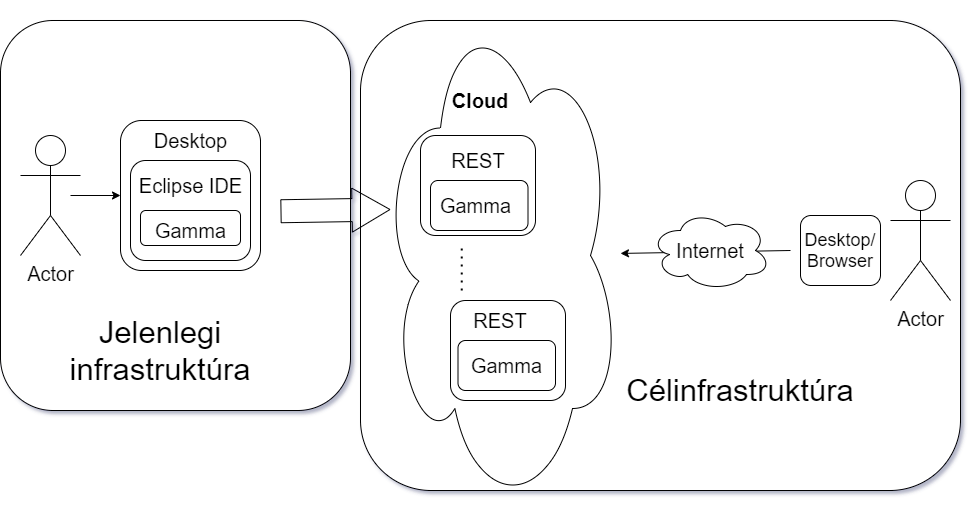
\includegraphics[width=150mm, keepaspectratio]{figures/transformation.png}
	\caption{Gamma mint szolgáltatás}
	\label{fig:transformation}
\end{figure}


Alapvetően a Gammát mint Eclipse IDE Plug-in ki kell emelni, hogy egy fekete szoftver doboz legyen, ami bemeneti paraméterként kap egy műveleteket leíró fájlt, ezután legyártja a különböző műveletek által definiált eredmény fájlokat. A Gamma fölé kell építeni egy webes kiszolgálót, ami képes bejövő kéréseket értelmezni, majd átfogalmazva továbbküldi a Gamma komponensnek. A megoldás során olyan mellék/segítő komponenseket is meg kellet tervezni és implementálni, amelyek az adatok átalakításáért vagy mozgatásáért felelősek.

%----------------------------------------------------------------------------
%\section{Motiváció}
%----------------------------------------------------------------------------

A felhő világban definiáltak alapján a rendszerünk egy \textbf{Software as Service (SaaS)} komponens lesz, amely megoldási szolgáltatás a leggyakrabban használt, röviden annyit foglal magába, hogy egy alkalmazást teszünk elérhetővé felhasználók számára az internet segítségével.
A rendszerünk felhőbe való integrációja mögötti igényt az alábbi három kategóriába sorolt előnyhalmaz magyarázza meg \cite{top10,ibm}:

 \begin{itemize}
	\item \textbf{Flexibilitás} : Igény szerint skálázható, publikus és privát adattárolás lehetősége, vezérlési lehetőségek (egy szervezet eldöntheti, hogy milyen szinten szeretné kontrollálni az igényelt szolgáltatását), gazdag portfólió (számos létező eszköz és megoldás közül választhatunk) és nem utolsó sorban biztonsági szempontból is rengeteg létező vagy új megoldást lehet implementálni az adatok titkosításához.
	\item \textbf{Hatékonyság} : Bárhonnan elérhető egy szolgáltatás az interneten keresztül, idő megtakarítás szempontjából a fejlesztők gyorsabban tudnak dolgozni, Hardware biztonság (egy esetleges hardware meghibásodás során nem veszítünk adatokat, anyagi megtakarítás), vállalatoknak nincs szüksége szerverekre és más hasonló felszerelésre.
	\item \textbf{Stratégiai érték} : Számos terhet vesz le egy felhőalapú szolgáltatás a szervezetek válláról, így több idő marad a fejlesztésekre, mindig friss az igénybe vett szolgáltatás verziója. Az elérhetőség lehetővé teszi, hogy a világ bármilyen részéről emberek közösen tudjanak dolgozni ugyanazon a problémán.
\end{itemize}

Mivel az alkalmazásunk egy webes szolgáltatás lesz, így ezzel az aspektussal járó pozitívumok is alátámasztják a rendszer piaci igényét.

Egy webes szolgáltatás lehetővé teszi, hogy a meglévő szoftverünket elérhetővé tegyük a világ számára \cite{tutorialspoint}. HTTP protokollt használva nem csak kliensek felé oszthatjuk meg, hanem különböző más létező szoftver komponensekkel való kommunikációt is kitudunk alakítani.
Rengeteg már létező megoldási minta létezik, így nehéz elakadni. Jól előredefiniált protokollok vannak meghatározva, így két teljesen különböző ipari ágakból származó rendszerek közti kommunikáció is kialakítható.

%----------------------------------------------------------------------------
%\section{Dolgozat felépítése}
%----------------------------------------------------------------------------

A szakdolgozat keretein belül a fentebb leírt megoldás specifikációját, fejlesztési folyamatát, tesztelési útmutatóját és továbbfejlesztési lehetőségét részletezem.
A következő fejezetben bemutatom az általam választott technológiákat amelyekkel a feladatot megoldottam, itt többek közt bemutatásra kerülnek a OSGi, Eclipse RCP és REST API fogalmak. Továbbá, specifikálom a feladatot, megfogalmazott követelményeket mutatok be és végigvezetem a fejlesztési folyamaton és felmerülő nehézségek megoldásában az olvasót. Ezt követően bemutatom a fejlesztést egy konkrét példa segítségével, zárásként pedig a továbbfejlesztési lehetőségekről fogok beszámolni.






















\numberwithin{figure}{section}

%----------------------------------------------------------------------------
\chapter{Háttér ismeretek}
%----------------------------------------------------------------------------
\section{Modern technológiák}
%----------------------------------------------------------------------------

A megoldás folyamán számos modern technológia bevezetésére, implementációjára volt szükség,  ezek közül a legfontosabbak:

%----------------------------------------------------------------------------
\subsection{OSGi}
%----------------------------------------------------------------------------

Az OSGi (Open Services Gateway Initiative) egy Java keretrendszer, amely segítségével moduláris szoftvereket és könyvtárakat tudunk fejleszteni.

A technológia alapvetően egy specifikáció halmazból, referencia implementációkból és minden specifikációhoz tartozó teszt halmazból áll össze, mindezek együtt leírnak egy dinamikus moduláris rendszert. A bevált szolgáltatás modellje lehetővé teszi, hogy az infrastruktúra és az alkalmazás komponensek úgy lokálisan, mint hálózaton keresztül is kommunikáljanak egymással, hogy egy koherens és konzisztens architektúrát alkossanak.

Az ipar bármely területén megtaláljuk az IoT-tól kezdve a telekommunikációs megoldásokig, viszont számos esetben nincs kiemelve, azaz ritkán van feltüntetve a használt technológiák listáján. 

Kompozícióilag két részből áll az OSGi. Az első egy olyan specifikáció, ami a moduláris egységeket írja le, ezeket bundle-knek vagy plug-in-eknek nevezzük. A specifikáció leírja, hogy milyen infrastruktúra szükséges az említett bundle-k számára és, hogy egyes bundle-k milyen életcikluson mennek át (Telepítve, Elindítva, Aktív, Elakadt, Felfüggesztett), továbbá meghatározza, hogy milyen kapcsolat lehet egyesek bundle-k közt és ezek hogyan kommunikálhatnak egymással. A második pedig egy JVM szintű nyilvántartó, amibe minden bundle tud bejegyzéseket tenni, hogy neki milyen publikálni kívánt objektumai vannak.


Az OSGi a fejlesztési ciklus majdnem minden területén csökkenti a komplexitást. Kódírás és tesztelés jelentősen kevesebb erőforrást fog elnyelni, támogatja az újrahasznosítást (létező komponenseket egyszerűen fel lehet használni egy új modulban). Az üzemeltetési feladatokat is könnyíti, lehetővé teszi a moduláris frissítést vagy telepítést, nem kell minden funkció bevezetésekor az egész rendszert leállítani. Könnyebben lehet lokalizálni egyes hibákat, így a támogatói feladatkör is egyszerűsödik. Az alkalmazásunk moduláris függőségi fájában egyszerűbben tudunk bizonyos elemeket bevezetni, helyettesíteni vagy akár kivenni.

További részletes leírást az OSGi specifikációban lehet olvasni:  \textbf{\href{https://www.osgi.org/developer/specifications/}{OSGi Specification}}

Eclipse világban az Equinox OSGi implementációt lehet használni, a fentebb részletezett szolgáltatásokat és szükséges infrastruktúrát alakítja ki számunkra.

%----------------------------------------------------------------------------
\subsection{Eclipse Plug-in fejlesztés}
%----------------------------------------------------------------------------

Eclipse egy nyílt forráskódú, platform független fejlesztői környezet (IDE). Egy alap munkaterület (workspace) és egy plug-in rendszert tartalmaz, aminek segítségével könnyen tesztre szabhatóvá lehet tenni. Az utóbbit használja ki a Gamma is és az általa használt mellék komponensek is. 

Az Eclipse IDE egy speciális Eclipse alkalmazás ami lehetővé teszi a fejlesztőknek, hogy egyedi alkalmazásokat tudjanak fejleszteni. Egy Eclipse alkalmazás egy vagy több szoftver komponensből tevődik össze ezeket nevezünk plug-in-eknek. Ezek a modulok bővíthetőek vagy felhasználhatóak más komponensek létrehozására. Összefoglalva, az Eclipse IDE egy több plug-in-ekből (JDT) álló Eclipse alkalmazás.

Lehetőségünk van az így létrehozott alkalmazásainkat összecsomagolni és az Eclipse IDE- től függetlenül futtatni és tesztelni (\textbf{headless Eclipse}).
Ehhez definiálnunk kell egy termék leírást (product configuration), aminek tartalmaznia kell az alkalmazásunk plug-in-jét, minden felhasznált függőséget és minden más olyan konfigurációt ami szükséges ahhoz, hogy egy külön komponenseként tudjuk hordozni a szoftverünket. Ilyen konfigurációk, az alkalmazás belépési pontja (extension point), komponensek indulási sorrendje, esetleges ikonok és függőségi fa, ami meghatározza, hogy milyen komponens mitől és hogyan (kötelező, opcionális) függ valamilyen más modultól.

A termékleírásunk egy alkalmazás osztályra kell mutasson ami alapértelmezetten két fajta lehet:

\begin{lstlisting}[language=]
org.eclipse.ui.ide.workbench - IDE alapú alkalamzások

org.eclipse.e4.ui.workbench.swt.E4Application - RCP alkalmazások, függetlenek az IDE-től
\end{lstlisting}

Ezektől el lehet térni és egy teljesen egyedi alkalmazást írni, ehhez a következő interfészt kell implementálni és behivatkozni a termék konfigurációnkba :

\begin{lstlisting}[language=]
org.eclipse.equinox.app.IApplication
\end{lstlisting}

A dolgozatban leírt fejlesztés ezzel a megoldási opcióval lett megvalósítva.

%----------------------------------------------------------------------------
\subsection{REST API}
%----------------------------------------------------------------------------

Az internet megszületése óta, mikor Charley Kline és Bill Duvall összekötöttek két számítógépet és elküldték egymásnak az "L" és "O" karaktereket, számos internet alapú adatmozgatási megoldás született ilyenek a CORBA, RPC vagy SOAP. Ezek mind nagyon komplex mechanizmusok és a mai világban elavultnak számítanak. Itt jön szóba a REST a legújabb iteráció az internetes adatszállítási megoldások körében.

REST vagy \textbf{RE}presentational \textbf{S}tate \textbf{T}ransfer egy tervezési stílus, amellyel különböző rendszerek közti kapcsolatot tudunk megvalósítani. Olyan rendszereket, amelyek megfelelnek a REST szabványnak RESTful rendszereknek is nevezünk, alapvetően ezeket két fő jellemző írja le, az első, hogy nem tartják nyilván az egyes kérések állapotát, a második pedig az, hogy elkülönítik a kliens és szerver fogalmakat. 

\begin{figure}[!ht]
	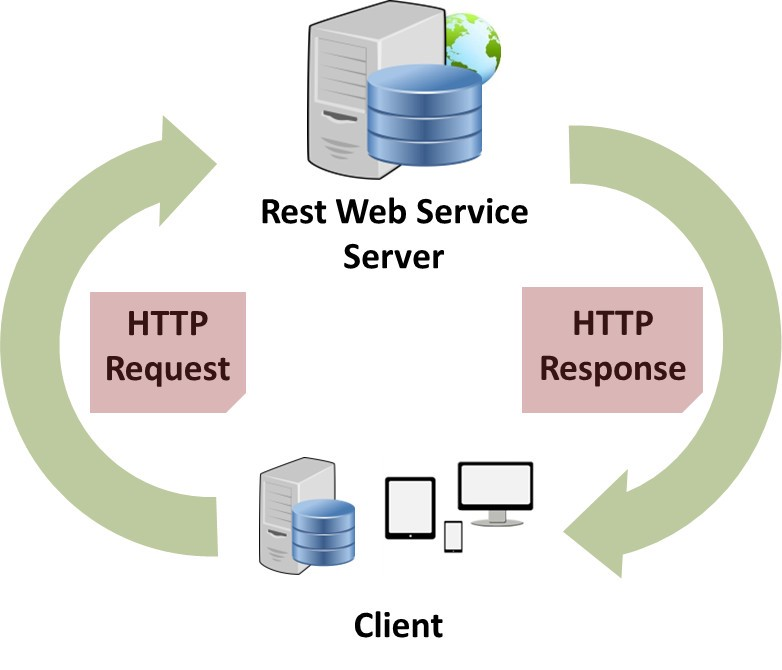
\includegraphics[width=150mm, keepaspectratio]{figures/rest_structure.jpeg}
	\caption{REST egyszerű architektúra}
	\label{fig:rest_structure}
\end{figure}

Ahhoz, hogy egy szolgáltatást RESTful-nak nevezzünk meg kell felelni egy szabványnak ami hat alapelvből áll.

 \begin{itemize}
	\item \textbf{Szerver és Kliens szeparáció} - a tervezési minta előírja, hogy a szerver és a kliens két független és önállóan egységként létező komponens kell legyen. Ez lehetővé teszi, hogy a két rendszerünket külön tudjuk fejleszteni, telepíteni, javítani, karban tartani. Bármilyen kódmódosítást kell végezni bármelyik oldalon a másikat nem befolyásolja mind addig amíg az interfész nem módosul, ilyenkor a szerver egy master szerepet vesz át és az elvégzett módosítást kezelni kell kliens oldalon is. Ez az elv támogatja a moduláris gondolkodást, ezzel flexibilissé válik a komplex rendszerünk. Továbbá, skálázhatósági lehetőségek is felmerülnek, hiszen az erőforrás igényesebb komponens alatti erőforrásokat igény szerint bővíthetjük. A szétválasztás lehetővé teszi, hogy akár egy szerverhez több kliens is csatlakozzon, így sokszínű rendszereket tudunk létrehozni. Ennek egy vizuális reprezentációja \aref{fig:rest_structure} ábrán látható.
	\item \textbf{Állapot nélküliség} - Ez az alapelv annyit von magában, hogy a szerver semmilyen információval nem rendelkezhet a kliens állapotáról ennek a kijelentésnek viszont fordítva is teljesülnie kell, azaz a kliens se ismerheti a szerver állapotát. Minden küldött/kapott üzenet egységként lehet kezelni, független attól, hogy a múltban milyen jellegű üzenet váltások történtek. Ennek eredménye az, hogy a csak kliens tárolja a saját adatainak az állapotát (nem a szerver adatait).
	\item \textbf{Egységes interfész} - Ez az alapelv négy szabályt határoz meg:
	\begin{enumerate}
		\item A kliens által kezdeményezett kérésnek tartalmaznia kell a fent definiált erőforrásnak az azonosítóját. Az erőforrást (egyed/objektum) hívhatjuk a webes kontextus alanyának is.
		\item A szerver válasza elegendő információt kell tartalmazzon az erőforrásról, pontosabban annyit, hogy a kliens tudja majd módosítani ezt.
		\item Minden egyes hívás az API felé részletes és tartalmilag teljes kell legyen. Továbbá a szerver válaszának is tartalmaznia kell elegendő információt, úgy, hogy a kliens értelmezni tudja ezt.
		\item Az utolsó szabálytól gyakran eltekintenek a fejlesztők, ez azt mondja, hogy a válasz, ami a szervertől érkezik tartalmazhat, olyan útmutatókat a kliens számára amivel az alkalmazás állapotát módosítani tudja. Például, ha egy objektumot lekér a kliens az API-tól, akkor a szerver a válaszba becsomagolhat olyan mellékes információkat amelyek azt írják le, hogy milyen módon módosítható a visszaadott objektum.
	\end{enumerate}
	Az egységes interfész lehetővé teszi, hogy a kliens típusától (böngésző, alkalmazás) eltudjunk tekinteni a szerver oldalon.
	\item \textbf{Cache lehetőség} - Cache támogatást úgy lehet elérni, hogy az adatokat verziózzuk, ha a kliens lekér egy adatot akkor valamilyen metaadatban tároljuk azt is, hogy ez milyen verziójú, így ha ugyanazt az objektumot szeretné lekérni, előtte tudja ellenőrizni lokálisan, hogy már a legfrissebb adattal rendelkezik és nem kell a szervert megint megszólítania. Ezzel terheléscsökkentést tudunk elérni.
	\item \textbf{Rétegelt architektúra} - A szerver és az erőforrást lekérő kliens között számos más rendszer helyezkedhet el, ezek többfajták lehetnek de legtöbbször a biztonsági, cache, terhelés egyensúlyozó rétegekkel találkozhatunk.
	\item \textbf{Igény szerinti kód (opcionális)} - Az egyedüli elv ami opcionális, annyit von magában, hogy a kliens bármikor kérhet kódrészleteket a szervertől és ez a válaszban valamilyen HTML vagy szkript formátumba becsomagolja és elküldi ennek , amit majd a kliens futtatni tud. Az alapelv teljesülése nélkül is tud egy rendszer RESTful lenni.
\end{itemize}

A fentebb többször említett kérés/válasz fogalmakat a REST világban HTTP kérésekbe csomagoljuk, ezek tipikusan a következőket kell tartalmazzák :
\begin{enumerate}
	\item egy HTTP ige, ami leírja a művelet típusát, jelenleg használt igék:
	\begin{enumerate}
		\item \textbf{GET} erőforrást tudunk lekérni, nagyon fontos, hogy nem módosíthat állapotot a szerveren
		\item \textbf{POST} erőforrás létrehozásra használják, többszörös hívás esetén különböző erőforrásokat fog létrehozni
		\item \textbf{PUT} már létező erőforrások állapot frissítésére használják, többszörös hívás ugyanazt kell, hogy eredményezze
		\item \textbf{DELETE} mint ahogy a neve is sugallja, erőforrás törlésre használják 
		\item \textbf{PATCH} parciális frissítési műveletekre tudjuk használni
		\item a maradék HTTP igéket nem szokták gyakran implementálni a REST világban
	\end{enumerate} 
	\item fejléc, ami metaadatokat tartalmaz az üzenetről, többek közt olyan jellegű információkat, mint az üzenet hossza, a tartalom típusa, a válasz HTTP kód száma és üzenete.
	\item az erőforrás elérési útja
	\item opcionális üzenettörzs, ami további adatot tartalmazhat
\end{enumerate}


%----------------------------------------------------------------------------
\subsection{OpenAPI és Swagger}
%----------------------------------------------------------------------------
\textbf{OpenAPI Specifikáció} egy API leíró szintaktika REST API-k számára. A specifikáció YAML és JSON formátumban is írható, az így létrehozott fájl a teljes API-t meghatározza, jellemzően a következőket tartalmazza:
\begin{itemize}
	\item Endpointok halmazát és az ezeken meghatározott műveletek leírását, mint például GET /api/students, ami a tanulók listáját adja vissza vagy a POST /api/students, ami a kliens oldalról felküldött adatok alapján létrehoz egy tanulót a szerver oldalon.
	\item Műveletek bemeneti és kimeneti paraméterét
	\item Autentikációs metódusokat
	\item Licenc, felhasználói feltételek vagy bármilyen adminisztratív információ ami az API-hoz tartozik
\end{itemize}

Az OpenAPI specifikációt korábban Swagger specifikációnak hívták, amíg a SmartBear Software felajánlotta az OpenAPI iniciatívának. Azóta az OpenAPI 3.0 verziónál tartunk, az új verzió részletes dokumentációjáról és az OpenAPI-ról itt lehet részletesebben információkat olvasni: \textbf{\href{https://www.openapis.org/blog/2017/07/26/the-oai-announces-the-openapi-specification-3-0-0}{OpenAPI 3.0 Documentation}}

\begin{figure}[!ht]
	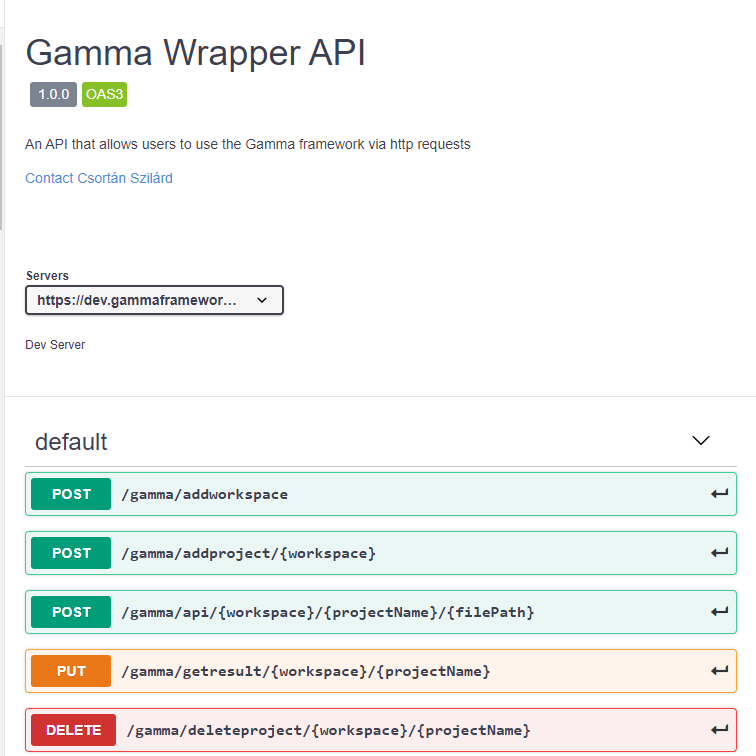
\includegraphics[width=150mm, keepaspectratio]{figures/swagerr_UI.png}
	\caption{Gamma OpenAPI Specification}
	\label{fig:openAPI_swagger}
\end{figure}

A Swagger egy olyan eszköztár ami az OpenAPI köré épült, hogy segítse a REST API tervezést, implementálást, tesztelést. Számos ilyen eszköz tartozik ide, ezek közül a legfontosabbak:
\begin{itemize}
	\item \textbf{\href{https://editor.swagger.io/?_ga=2.32011518.1535494714.1606415394-1420243541.1606415394}{Swagger Editor}} Egy böngészőből elérhető felhasználó barát felületet biztosít, ahol lehetőségünk van megírni a specifikációnkat. Számos előnyt kínál egy hagyományos szerkesztőhöz képest, ilyenek a szintaktikai ellenőrzések, bizonyos REST API szabályok betartását is megköveteli, pl: egy GET metódusnak nem lehet törzse.
	\item  \textbf{\href{https://swagger.io/swagger-ui/}{Swagger UI}} Egy olvasható, részletes és vizuálisan látványos dokumentációt generál az Editorban elkészített API specifikációnkhoz, \aref{fig:openAPI_swagger} ábrán egy ilyent lehet megtekinteni.
	\item  \textbf{\href{https://github.com/swagger-api/swagger-codegen}{Swagger Codegen}} Kliens oldali könyvtárakat és szerver oldali keretet tud generálni.
\end{itemize}

A specifikációnak tehát rengeteg előnye van, többek közt az egységes API leírás, ami platform független, a kódgenerálás miatt több erőforrás marad az üzleti logika implementálásra vagy  az automatizált dokumentáció készítés.
%----------------------------------------------------------------------------
\subsection{Fontosabb Java könyvtárak}
%----------------------------------------------------------------------------
A Vert.x egy eszköztár, amelynek segítségével JVM alapú alkalmazásokat tudunk készíteni. Nagyon flexibilis, azaz nagyon széles az alkalmazás típus spektrum, ahol használni lehet. HTTP/REST mikroszolgáltatások, komplex webes alkalmazások vagy eseményvezérelt back-end fejlesztése során is használható.

Flexibilitása miatt a piac számos területén használjak, például valós idejű játékokban vagy banki rendszerekben.

JVM alapú programozási nyelvek bármelyikében használható (Java, Kotlin, JavaScript, Groovy, Ruby, Scala).

OpenAPI specifikáció integrálását is támogatja. Nagyon egyszerűen lehetőségünk van behivatkozni az API-t leíró fájlunkat, ami alapján a Vert.x legenerál egy interfész réteget, amely mögé nagyon egyszerűen letudjuk implementálni az üzleti logikánkat.
%----------------------------------------------------------------------------
\section{Gamma}
%----------------------------------------------------------------------------

A Gamma egy tanszéken fejlesztett eszköz, amely segítségével komponens alapú reaktív rendszereket tudunk modellezni. Több funkcióval rendelkezik, ezek kerülnek rövid bemutatásra ebben a fejezetben, részletes dokumentációt számos publikáció tartalmaz ezekről itt lehet olvasni: \textbf{\href{https://inf.mit.bme.hu/node/6028}{Gamma Keretrendszer}}
%----------------------------------------------------------------------------
\subsection{Gamma funkciók}
%----------------------------------------------------------------------------
Támogatott mérnöki modellek integrációja \textbf{modell transzformáció}  segítségével történik. Ez a funkció egy létező mérnöki modellt fordít le a Gamma állapotgép nyelvére, ezzel a felhasználót segíti, mivel automatizálva történik a forrás nyelv és a gamma közti leképezés. Jelenleg a Yakindu és UPAAL modellezési nyelveket képes a Gamma transzformálni, viszont a plug-in koncepció további nyelvek leképezését is lehetővé teszi.

A \textbf{validáció} egy statikus analízis technika, mely visszajelzést ad a létrehozott modellek szintaktikai helyességéről. A Gamma az önálló modelleken és a kompozit állapotgép komponenseken is végez validációt.

A Gamma képes Java programozási nyelvre \textbf{automatizáltan kódot generálni}. Interfész definíciókat a Gamma interfészekből generálja a funkció, a komponens implementációkat pedig a kompozit állapotgép modellezés során definiáltak alapján készíti el.

Két \textbf{verifikáció} funkcionalitást támogat a Gamma :
\begin{itemize}
	\item formális verifikáció, amely formális modellezési nyelvek integrációjával valósul meg. Jelenleg a Gamma keretrendszerbe az UPAAL van integrálva.
	\item back-annotation, amely felhasználja a formális verifikáció eredményét és ezt felhasználva  generál egy végrehajtási láncot amely alátámasztja vagy megcáfolja az egyes rendszer követelményt.
\end{itemize}

A Gamma az UPAAL modell ellenőrzőt felhasználva képes \textbf{teszteket generálni}, ehhez létrehoz egy absztrakt Gamma modellt, amely alapján legenerálja a teszt eseteket.

%----------------------------------------------------------------------------
\subsection{Gamma hiányosságok} \label{gamma_missing}
%----------------------------------------------------------------------------

A Gamma egy Eclipse IDE-ben létező keretrendszer, így jelentős kihívást jelent, hogy egy felhasználó kipróbálja esetleg használja. Kezdve az Eclipse világ rejtelmeitől a különböző függőségi nehézségekig számos hibalehetőség lép föl, ha használni szeretnénk az alkalmazást. Továbbá, vannak olyan modellek amelyek több ezer akár millió nagyságrendű állapottal rendelkeznek, ilyen modelleken a fentebb leírt műveletek futtatása igenis erőforrásigényes. Sajnos az IDE-hez kötöttség nem segít ezen problémák megoldásában, nehéz a skálázhatóság és a disztribúció kérdésekre választ kapni jelen kontextusban.














%----------------------------------------------------------------------------
\chapter{Specifikáció és implementáció}
%----------------------------------------------------------------------------

Ez a fejezet tartalmazza a \ref{gamma_missing} fejezetben leírt hiányosságokra adott megoldásom specifikációját, architektúra tervét és implementációját. 

%----------------------------------------------------------------------------
\section{Specifikáció}
%----------------------------------------------------------------------------

A specifikálást a rendszert meghatározó követelmény halmaz kialakításával kezdjük. A követelményeket alapvetően két csoportra lehet osztani, funkcionális és nem funkcionális. Kulcsfontosságú absztrakt követelményeket az alábbi lista foglal össze, viszont nem tartalmazza a teljes körű követelmény hierarchiát, ezt \aref{fig:requierments_placeholder} és \aref{fig:requierements_2} ábrákon lehet megtekinteni.

\begin{itemize}
	\item A rendszer képes kell legyen a gamma modelleket és a hozzá tartozó adatokat tartalmazó eclipse projektek kezelésére.
	\item A felhasználónak lehetősége kell legyen felküldeni a rendszer számára a saját eclipse projektjeit.
	\item A felhasználónak lehetősége kell legyen a saját felküldött projektjein gamma műveleteket futtatni.
	\item A felhasználónak lehetősége kell legyen a gamma művelet eredményeit lekérni a rendszerünktől.
	\item A rendszer képes kell legyen felhasználók azonosítására.
	\item A rendszer képes kell legyen inaktív projektek automatizált törlésére.
\end{itemize}

\begin{figure}[t]
	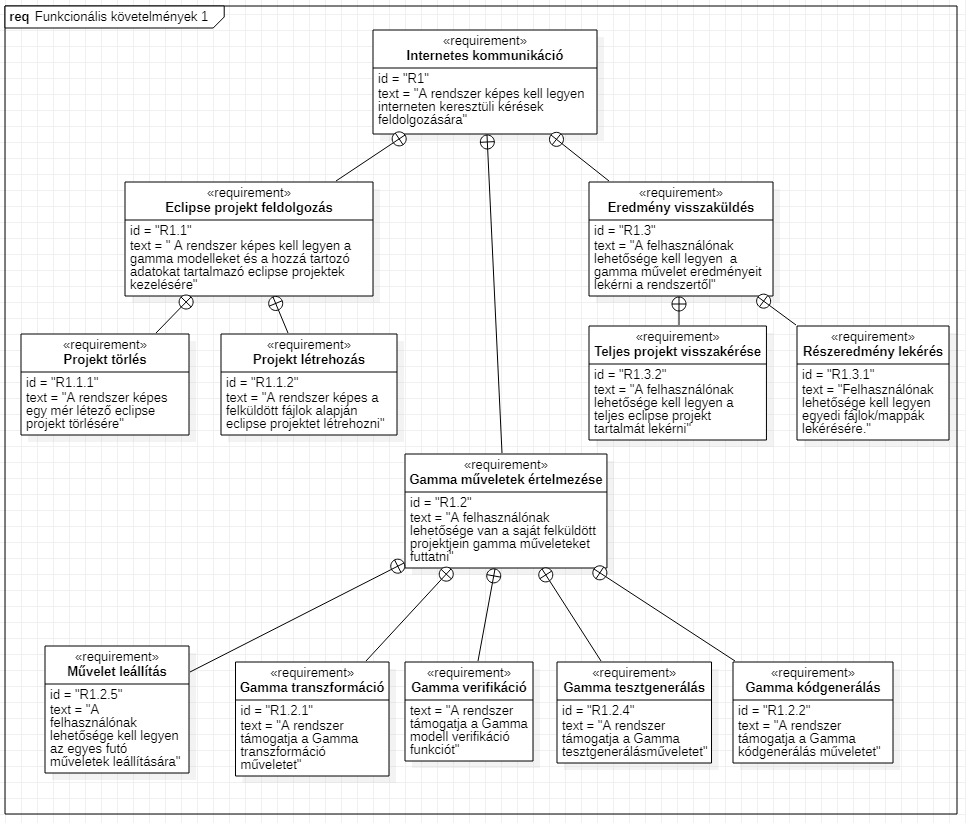
\includegraphics[width=\textwidth, keepaspectratio]{figures/requierments_placeholder.png}
	\caption{Követelmény hierarchia 1}
	\label{fig:requierments_placeholder}
\end{figure}

\begin{figure}[t]
	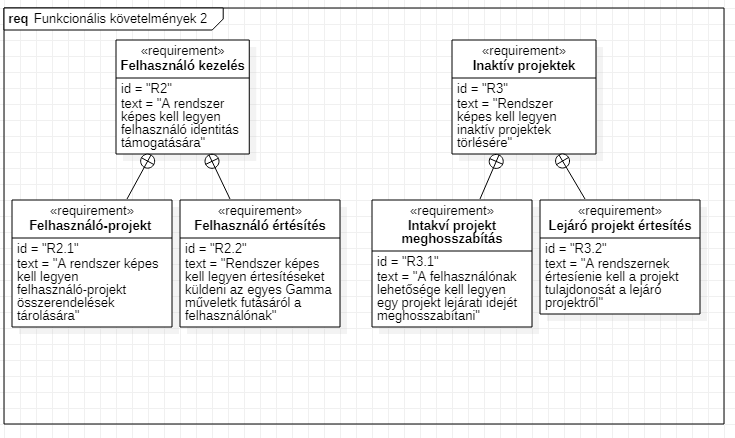
\includegraphics[width=150mm, keepaspectratio]{figures/requierments_2.png}
	\caption{Követelmény hierarchia 2}
	\label{fig:requierements_2}
\end{figure}

A további nem funkcionális követelményeket négy kategóriába soroljuk:
\begin{itemize}
	\item \textbf{Megbízhatóság:} Egy projekten nem futtathatunk két különböző Gamma művelet halmazt
	\item \textbf{Biztonság:} Minden felhasználó csak a saját projektjeit szerkesztheti / saját projektjein futtathat gamma művelet halmazokat / A rendszer képes kell legyen kiszűrni az egyes rosszindulatú felhasználók által megadott fájl elérési utakat / 
	\item \textbf{Teljesítmény:} A rendszer képes kell legyen különböző projekteken ugyanabban az időben Gamma műveletek futtatására. / A rendszer skálázható kell legyen. / A rendszernek nem szabad fölösleges adatot tárolnia. / A rendszer muszáj töröljön minden olyan adatot, amely neki vagy a felhasználó számára nem releváns. / A rendszer képes kell legyen asszinkron módban működni.
	\item \textbf{Felhasználhatóság:} A rendszer megfelelő, HTTP szabvány által előírt válaszokat adni az egyes kérésekre. / A rendszer beszédes értesítéseket kell küldjön a projekt tulajdonosának az egyes Gamma műveletek futási állapotáról.
\end{itemize}

A fentebb leírt követelmények alapján bizonyos technológiai döntéseket kellet hozni a projekt iniciális fázisaiban. Ahhoz, hogy az alkalmazásunk interneten keresztül is elérhető legyen egy webszervert kellet kialakítanunk, ez lesz a rendszer belépési pontja. A webszerver a REST API modern architektúra stílus szabályait betartva lett kialakítva. Mindez a \textit{R1.*} követelmény teljesítése teszi szükségessé. 

Ahhoz, hogy az \textit{R1.2.*} követelmény teljesüljön, a Gamma keretrendszert egy \textit{headless Eclipse}-be kellet becsomagolni. Ezzel megtudjuk oldani azt a problémát, hogy a Gamma az Eclipse IDE-hez van kötve, az így becsomagolt keretrendszert parancssoron keresztül lehet elérni.

Az \textit{R2.*} követelményt eclipse munkaterek (workspace) használatával teljesítjük. A rendszerünk biztosít munkatér létrehozás funkciót a felhasználói oldalon álló kliens szoftvernek, ehhez rendel egy egyedi azonosítót amit visszaküld a kliensnek és mostantól, ezzel az azonosító megadásával tud a kliens további funkciókat elérni. Mindezzel azt érjük el, hogy majdnem semmilyen információt nem kell tárolni a felhasználóról, ezt a feladatot rábízzuk a kliens szoftverre.

Összefoglalva a követelményeket és a technológiai döntéseket, olyan rendszert tervezünk, amely a Gamma keretrendszert elérhetővé teszi a világ számára, oly módon, hogy közben több felhasználói rendszerlogikát támogat az adatok tárolásán és funkciók elérésén. Továbbá, olyan mellék funkciókat is biztosítania kell, mint inaktív projektek automatizált törlése vagy felhasználók értesítése.

A rendszerben érdekelt személyek listája (\textbf{stakeholders}), azaz olyan aktorok, akik valamilyen módon kapcsolatba léphetnek a rendszerrel:
\begin{itemize}
	\item Komplex modellekkel foglalkozó \textbf{mérnökök} (NASA)
	\item \textbf{Egyetemi kutatók}
	\item Olyan \textbf{fejlesztő} aki integrálni akarja a rendszerünket egy harmadik párti alkalmazásba (MagicDraw)
	\item \textbf{Gamma fejlesztő} ,aki erőforrás igényes funkciót akar tesztelni
	\item \textbf{Üzemeltető}, aki a rendszer komponenseit frissíteni tudja
	\item \textbf{Üzleti oldalú kolléga}, aki a rendszert mint szolgáltatás hirdeti/eladja
\end{itemize}

A rendszer jelen formájában nem tartalmazza a fentebb többször említett kliens komponenst, így precíz használati eseteket nehéz definiálni. Ennek ellenére a rendszert teljes funkcionalitását lehet használni, tesztelni valamilyen API tesztelő szoftverrel, mint például PostMan. Olyan kéréseket tudunk küldeni az alkalmazás felé, amelyek teljes körűen szimulálják egy kliens szoftver viselkedését.

Az alapvető elérhető funkciók közé tartozik: a munkatér létrehozás, amely egy felhasználónak dedikált eclipse munkateret hoz létre, amin belül majd további műveleteket lehet végezni; eclipse projekt importálása archivált forrásból egy létező munkatérbe; az importált projektben szereplő, műveleteket leíró fájlok alapján gamma műveletek futtatása; a gamma műveletek által generált elemek visszakérése archivált fájlként; importált eclipse projekt törlése.


%----------------------------------------------------------------------------
\section{Architektúra}
%----------------------------------------------------------------------------

Ez a fejezet részletezi a specifikált rendszer struktúráját, továbbá áttekintünk fontosabb folyamatokat.
%----------------------------------------------------------------------------
\subsection{Struktúra}
%----------------------------------------------------------------------------

A rendszer felépítését \aref{fig:structure} ábra mutatja be. A továbbiakban részletezem az ábrán látható egyes komponenseket, milyen szerepük van és hogyan kommunikálnak más komponensekkel.
\begin{figure}[t]
	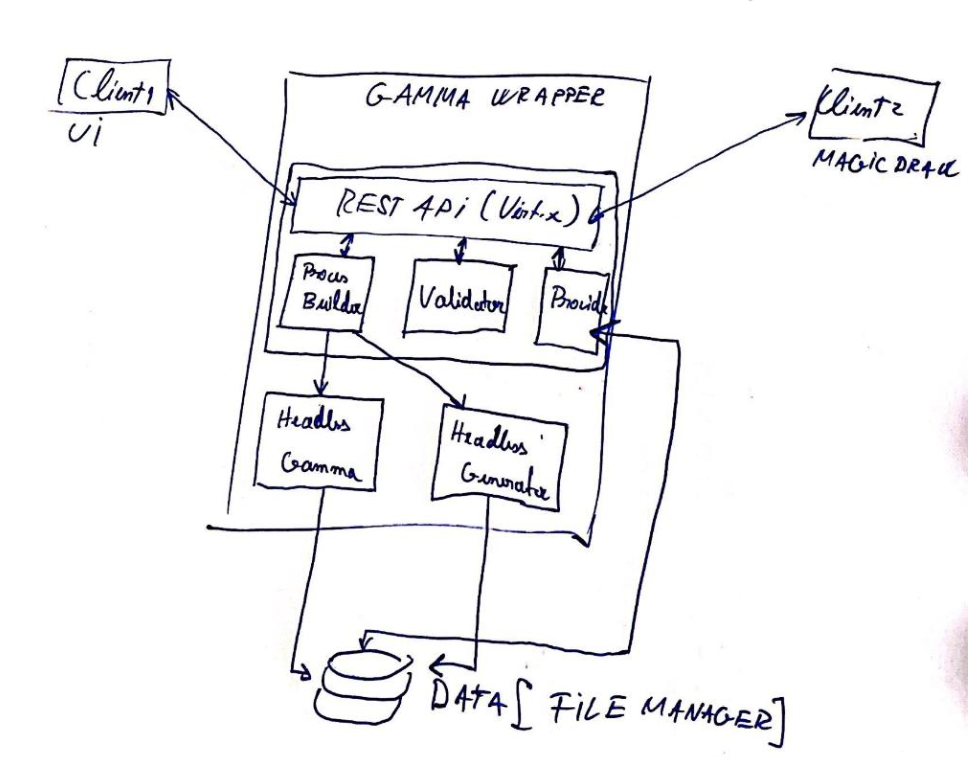
\includegraphics[width=150mm, keepaspectratio]{figures/architecture.jpg}
	\caption{Architektúra terv}
	\label{fig:structure}
\end{figure}
Az ábrán látható egy nagyobb, mindent magába foglaló \textit{Gamma Wrapper} nevezetű modul, ez a rendszer amely megvalósításra került a félév során és amiről a dolgozat szól. A nevét a funkcionalitásáról kapta, magyarul \textit{Gamma csomag}-nak is nevezhetnénk.

\paragraph{REST API} Ez az alkalmazás belépési pontja, ez látható a világ számára. Önmagában egy Vert.x webszerver amely egy OpenAPI specifikációban\footnote{OpenAPI specifikáció \url{https://app.swaggerhub.com/apis/szlnnn/GAMMA_WRAPPER3.0/1.0.0}} meghatározott \textit{endpoint}-ok alapján épül fel. Endpointnak hívjuk azokat az egyedi belépési pontokat, amelyek meghívhatók az alkalmazáson kívül. A rendszer az alábbi endpointokat tartalmazza, a fontosabbak működését a következő fejezet részletesen bemutatja:
\begin{itemize}
	\item POST /gamma/addworkspace eclipse workspace létrehozásának lehetőségét kínálja fel, minden további művelethez szükséges, a kérés nem tartalmaz további információt
	\item POST /gamma/addproject/{\textit{workspace}}\footnote{Minden döntött betűs rész egy URL-ben utazó paraméter} eclipse projekt létrehozást teszi lehetővé a {workspace} paraméterből kiolvasott munkatérben, a kérés törzsében szerepelnie kell az archivált fájl, ami tartalmazza az importálni kívánt projektet
	\item PUT /gamma/api/{\textit{workspace}}/{\textit{projectName}}/{\textit{filePath}} a munkatér és projekt páros alapján meghatározott Gamma műveleteket tartalmazó fájl futtatását teszi lehetővé. A {\textit{filePath}} paraméter írja le, hogy a műveleteket leíró fájl hol van, ez relatív kell legyen és a {\textit{projectName}} paraméterben tárolt projekt mappájában
	\item PUT /gamma/stopprocess/{\textit{workspace}}/{\textit{projectName}} a fentebb leírt folyamat leállítását teszi lehetővé, mivel egy projekt-munkatér pároson egy időben csak egy gamma művelethalmaz futhat ezért elég csak ezt a párost megadni
	\item PUT /gamma/getresult/{\textit{workspace}}/{\textit{projectName}} a gamma által generált fájlok visszakérését teszi lehetővé, ehhez szükséges, hogy a kérés törzsében utazzon, hogy milyen fájlokat/könyvtárakat szeretnénk visszakérni, az itt megadott elérések a projekthez képest relatívak kell legyenek, ha szerepel a "." elérés akkor a projekt teljes tartalmát visszaküldjük
	\item DELETE /gamma/deleteproject/{\textit{workspace}}/{\textit{projectName}} eclipse projekt törlését teszi lehetővé
	\item PUT /gamma/extendexpiration/{\textit{workspace}}/{\textit{projectName}} alapértelmezetten minden projekt automatikusan törlésre kerül 30 nappal a létrehozás után, ezzel az endpointal további 30 nappal lehet ezt az időtartamot meghosszabítani, az URL-ben utazó munkatér és projekt név párossal tudjuk eldönteni, hogy melyik projektet kívánja a felhasználó meghosszabbítani.
\end{itemize}
A komponens további feladatok is ellát, ilyenek a megfelelő HTTP válasz összeállítása, a szerverre küldött fájlok automatikus mentése vagy a más komponensek vezérlése. Egy időzítő is ide tartozik, ezzel ellenőrizzük a projektek lejárati dátumát és, ha ennek eljön az ideje akkor egy törlést fog indítani.

\paragraph{UI és MagicDraw} Mivel a rendszerünk egy szerver oldali komponens, ezért önmagában nem tudja bárki használni. Az ábrán feltüntetett kliens rendszereknek kell a felhasználói felület szerepét betölteni, ilyen lenne egy speciális UI ami az alapvető funkcióknak egy grafikus felületet biztosít és kontextust ad az alkalmazásunknak. Továbbá, tervben van a Gamma integrációja a MagicDraw\footnote{MagicDraw modellező eszköz \url{https://www.nomagic.com/products/magicdraw}} modellező eszközbe, a rendszerünk ezt az integrációt megkönnyítené. 

\paragraph{Headless Generator} A Gamma önmagában nem képes eclipse munkatér és projekt létrehozásra ezért kellet egy olyan komponens, ami előkészít egy környezetet, amiben futtathatunk Gamma műveleteket, ennek a neve \textit{Headless Generator}. Két fő funkciója van: eclipse munkatér (workspace) létrehozás és eclipse projekt importálás egy megadott munkatérbe. Mindkét funkcionalitást ugyanaz a folyamat valósítja meg annyi eltérésben, hogy ha a komponens kap egy archivált fájl elérést akkor tudni fogja, hogy ezt importálnia kell, mint eclipse projekt.  Egy \textit{headless runtime eclipse}-ként van megvalósítva és parancssorból lehet meghívni, két paramétert lehet megadni az első a \textit{-data} amiben a workspace nevét kell megadni, ha egy nem létező workspace-t adunk meg akkor a komponens ezt létrehozza, ez egy kötelező paraméter. A második argumentum pedig a projekt archivált fájl elérése, ezt fogja kicsomagolni és regisztrálni a munkatérbe, ez az argumentum opcionális. Fontos kiemelni, hogy a forrás fájl már a munkatér mappájában kell legyen.

\paragraph{Headless Gamma} Annak ellenére, hogy csupán egy endpoint meghívása során kerül működésbe a rendszer legfontosabb eleme. A Headless Generator-hoz hasonlóan egy headless runtime eclipse-ként lett kialakítva és ugyanúgy parancssorból lehet elindítani. Három kötelező paraméterre van szüksége. (1) Létező munkatér, amely tartalmazza az átadott (2) projekt állományait. Az utolsó (3) paraméter egy a projekthez relatív elérés, ami a gamma műveleteket leíró fájlra mutat. A fájl .ggen kiterjesztésű kell legyen, és megfelelő sorrendbe kell tartalmazza a futtatni kívánt műveleteket és a futtatáshoz szükséges modell állományok hivatkozását, amelyek a projekten belül kell legyenek. A Gamma miután elvégezte a műveleteket tipikusan 3 mappába generálja le az eredményeket: src-gen,test-gen, trace. Ezek mind a projekt mappán belül találhatóak. 

Az UPAAL telepítése egy alapvető követelmény a gamma megfelelő működéséhez, ennek az elérést a rendszer a környezeti változókból tudja kinyerni.
Az OSGi előnyeit itt tudjuk kihasználni, mivel a headless gamma több száz \textit{plug-in}-t igényel. A plug-in-ek egyesével frissíthetőek, elméletileg nem kéne nagy akadályt okozzon egy új release telepítése.

\paragraph{Process Builder} A REST webszerver és a headless komponensek közé biztosítani kell egy olyan réteget, ami a webes hívások paramétereit átalakítja parancssori argumentumokká és eltud indítani egy ilyen runtime eclipse-t, ezt a szerepet a \textit{Process Builder} tölti be. Négy funkció esetén jelenik meg a végrehajtási sorban, (1) munkatér létrehozás, (2) projekt importálás archív fájlból, (3) gamma művelet futtatás és (4) gamma műveletet futtató folyamat leállítás. Minden funkció esetén lehetőség van asszinkron működésre, viszont jelenleg csak a (3) és (4) esetén van implementálva,  a szinkron működést azzal az érvel lehet védeni, hogy csak abban az esetben küldjünk választ a kliensnek ha valóban a kért funkcionalitást eltudtuk végezni. Ez a gamma művelet futtatáskor azért nem egy élhető koncepció, mert vannak olyan modellek amelyek több ezer vagy akár több tíz ezer állapotból állnak, ezeknek a feldolgozása órákba is kerülhet így az asszinkron működés egy szükséglet. A gamma művelet leállítása pedig nem igényel semmilyen megvárást, nincs olyan eset amikor ez eltud akadni. A másik két esetben (1)(2) viszont megvárjuk amíg a munkatér vagy projekt létrejön, mert nem költséges műveletek, ezt a jövőben érdemes lehet átgondolni és esetleg átalakítani.
\paragraph{Validator} A valamennyi bejövő kérések validációs lépéseken is át kell essenek, ezt a \textit{Validator} modul biztosítja. A REST webszerver vezérli, hogy a bejövő paraméterek közül melyek azok amelyek valamilyen validáción át kell essenek. A legfontosabb ellenőrzési lépések közé tartoznak a munkatér létezés ellenőrzése, a projekt-munkatér páros vizsgálata és az átadott projekten futó gamma folyamat ellenőrzése. Az utóbbi kiemelkedően fontos, hiszen egy futás alatt levő projekttel nem végezhetünk semmit, csak leállíthatjuk. Ahhoz, hogy a futás állapotát nyilván tudjuk tartani, be lett vezetve egy leíró json fájl amit minden projekt importálásánál létrehozunk, ez a fájl többek közt tartalmazza azt is, hogy jelenleg van-e futó folyamat a projekten. Ennek az állapotát a ProcessBuilder beállítja \textit{inProgress}-be majd a HeadlessGamma futása végén frissíti \textit{notInProgress}-re.
\paragraph{Provider} A \textit{Provider}-nek két feladat van, az első, hogy a REST webszerver által feldolgozott eredmény visszakérő endpoint-ban megadott relatív elérések alapján összecsomagoljon egy zip állományt, a másik pedig a projekt törlés. Az eredmény fájl összecsomagolásánál lehetőségünk van megadni egyedi fájlok elérését vagy akár teljes mappákat. Ide tartozik a teljes projekt mappa is, ezt a "." eléréssel tudjuk megadni, ha ez szerepel a kérésbe akkor a többi eredmény eléréssel nem is foglalkozik a rendszer, hiszen ez mindent tartalmazni fog.
\paragraph{Data} Az ábrán megjelenik a \textit{Data} fogalom is, ez valójában a hoszt szerveren levő fájl kezelőt jelenti. Itt tároljuk a létrehozott munkatér és projekt párosokat és ezek teljes tartalmát, továbbá a metaadatokat tároló json fájlokat is. Egy adatbázis réteg bevezetésével a fájlban tárolt metaadatokat könnyebben tudnánk kezelni, sajnos a projektbe ez nem fért bele.



%----------------------------------------------------------------------------
\subsection{Folyamatok}
%----------------------------------------------------------------------------

Négy alapvető funkció részletes működését fogom bemutatni ebben a fejezetben, ezek sorra: munkatér létrehozás, projekt importálás, gamma műveletek futtatása és a futtatás eredmény lekérés. A folyamat bemutatja milyen modulokon megy végig az adat, továbbá milyen feldolgozások történnek egyes végrehajtási lépéseken. Mindezt szekvencia diagramokkal ábrázoltam. Az így bemutatott funkciók lefedik a rendszer legfontosabb felhasználói eseteit.


\paragraph{Munkatér létrehozás}

\begin{figure}[!ht]
	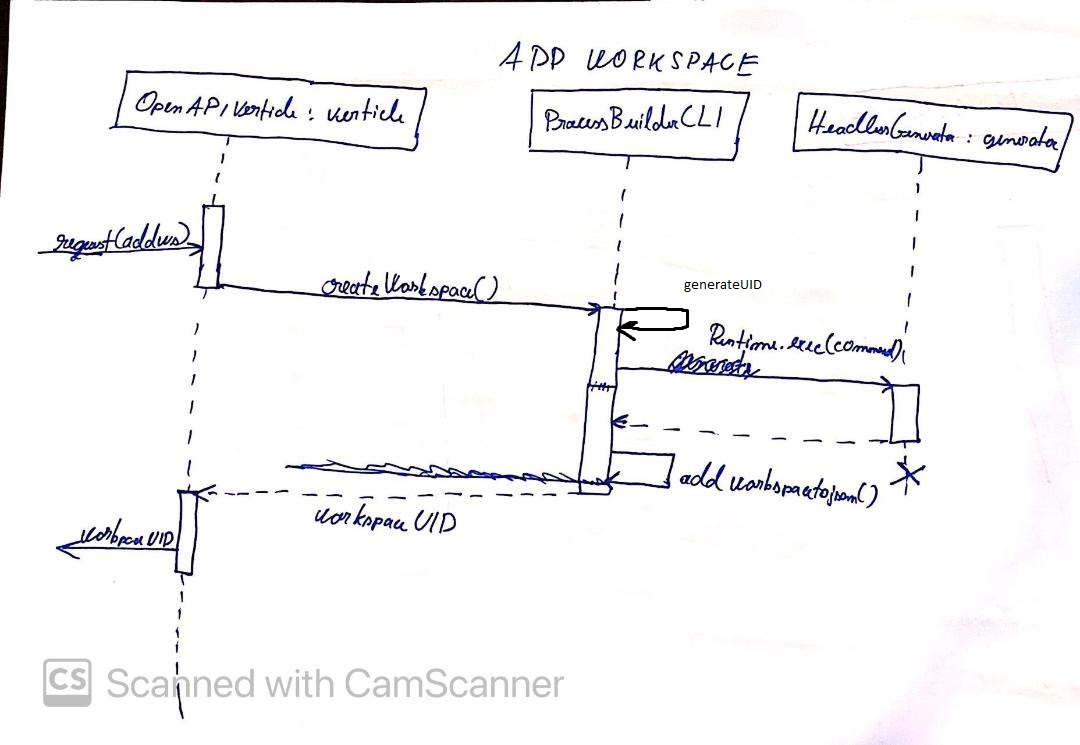
\includegraphics[width=150mm, keepaspectratio]{figures/add_workspace_seq.jpg}
	\caption{Munkatér létrehozás szekvencia diagram}
	\label{fig:addworkspace}
\end{figure}

A workspace létrehozás szekvencia diagramja \aref{fig:addworkspace} ábrán látható. Első fázisban bejön egy POST HTTP metódus az addworkspace endpointra, ennek a törzse üres és az URL-ben sem hordoz paramétereket. Látható, hogy az OpenAPIVerticle fogadja a kérést, ez lényegében a REST webszerverünk, mivel ez a legelső művelet, amit a kliens meg kell hívjon így nem kell semmilyen ellenőrzést végezni. A végrehajtási sor következő lépése a \textit{ProcessBuilder}-ben van, itt a rendszer generál egy egyedi UID azonosítót, amit felhasznál a parancs kialakításhoz, amivel elindítja a a HeadlessGenerator-t.A parancs (command) elkészítéséhez a ProcessBuildernek szüksége van a headless eclipse elérésére, ezt a \textit{config.properties} fájlban lehet beállítani. A generator amíg elkészíti a workspace-t a ProcessBuilder vár, ha végzett akkor visszaadja az OpenAPIVerticle-nek a generált UID-ot ami továbbítja a kliens felé. Mikor a headless eclipse elvégezte a feladatot akkor teljesen leáll, ezt jelzi az X a folyamatábrán.


\paragraph{Eclipse projekt importálás}
\begin{figure}[!ht]
	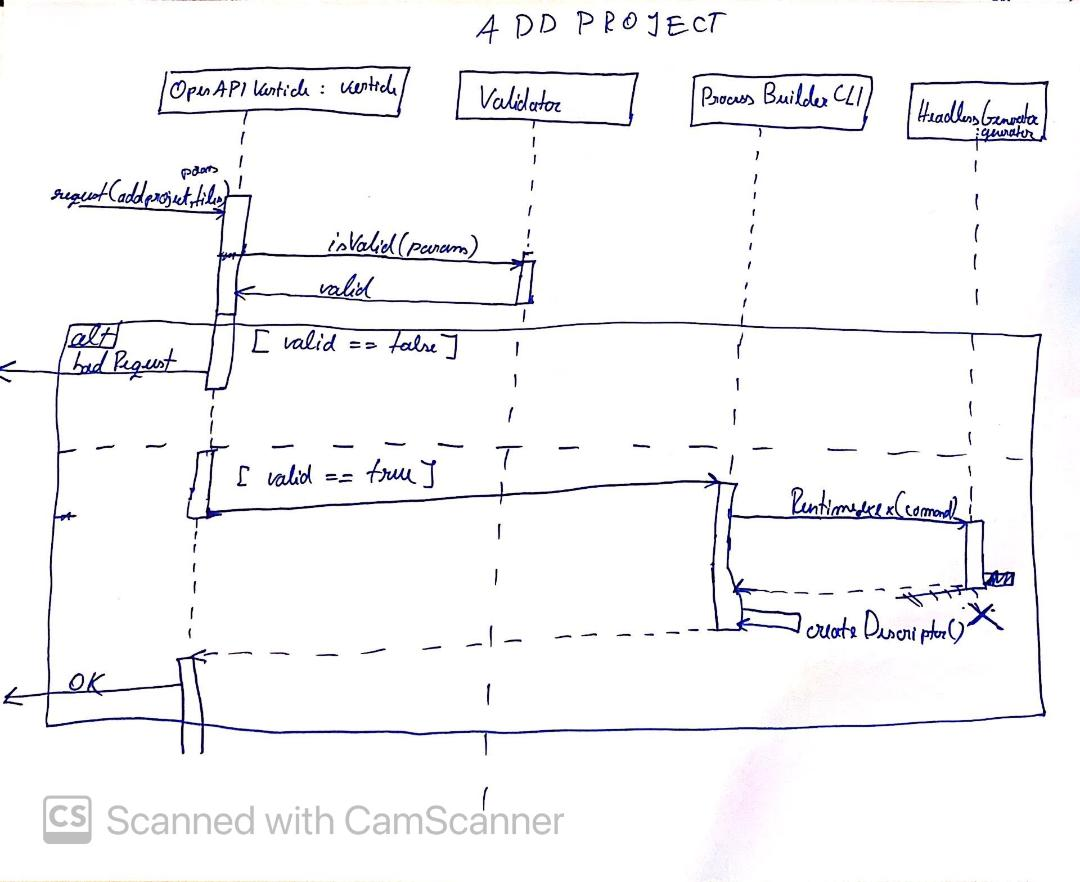
\includegraphics[width=150mm, keepaspectratio]{figures/add_eclipseproject_seq.jpg}
	\caption{Eclipse projekt importálás szekvencia diagram}
	\label{fig:addproject}
\end{figure}

A projekt importálás funkció szekvencia diagramját \aref{fig:addproject} ábrán lehet megtekinteni. A folyamat megint a kérés érkezésével indul, ezt minden esetben az OpenAPIVerticle dolgozza fel, ez a kérés egy POST HTTP metódus ami az addproject endpoint-ra jön be. Ebben az esetben viszont már az URL-ben utazik egy munkatér azonosító amit korábban adtunk vissza a workspace létrehozáskor. Továbbá, a törzsben két attribútum szerepel: (1) \textit{files} ez tartalmazza a projekt archivált állományait és (2) \textit{contact} ez egy email cím, ami a projekt tulajdonosáé, erre későbbiekben értesítések küldésénél lesz szükségünk. A munkatér létezését a Validator komponenssel elvégezzük, a kapott válasz alapján két esetet különböztetünk meg, az első, ha nem érvényes a megadott workspace azonosító, ekkor egyből szólunk a kliensnek, hogy rossz a kérés. Viszont, ha ez helyes akkor tovább adjuk a kérést a ProcessBuilder-nek ami az előző esethez hasonlóan elindítja a HeadlessGenerator-t, de kiegészíti az argumentum listát a forrás fájl nevével, mindezek előtt a nyers fájlt a munkatér mappájába másolja. A generator elvégzi az import műveletet, majd visszaadja a futási jogot a ProcessBuildernek, ami végezetül regisztrálja a munkatér-projekt párost és létrehoz egy leíró fájlt a frissen létrehozott projektben, ami tartalmazza, hogy mi a projekt neve, ki hozta létre (email cím), mikor hozta létre, mikor jár le és beállítja, hogy jelenleg nincs futás alatt, ezek után törli az iniciális forrás fájlt, hogy tárhelyet spóroljunk. Végezetül visszaadja a futási jogot a verticle-nek aki jelez a kliensnek, hogy minden rendben létrejött.



\paragraph{Gamma műveletek futtatása}
\begin{figure}[!ht]
	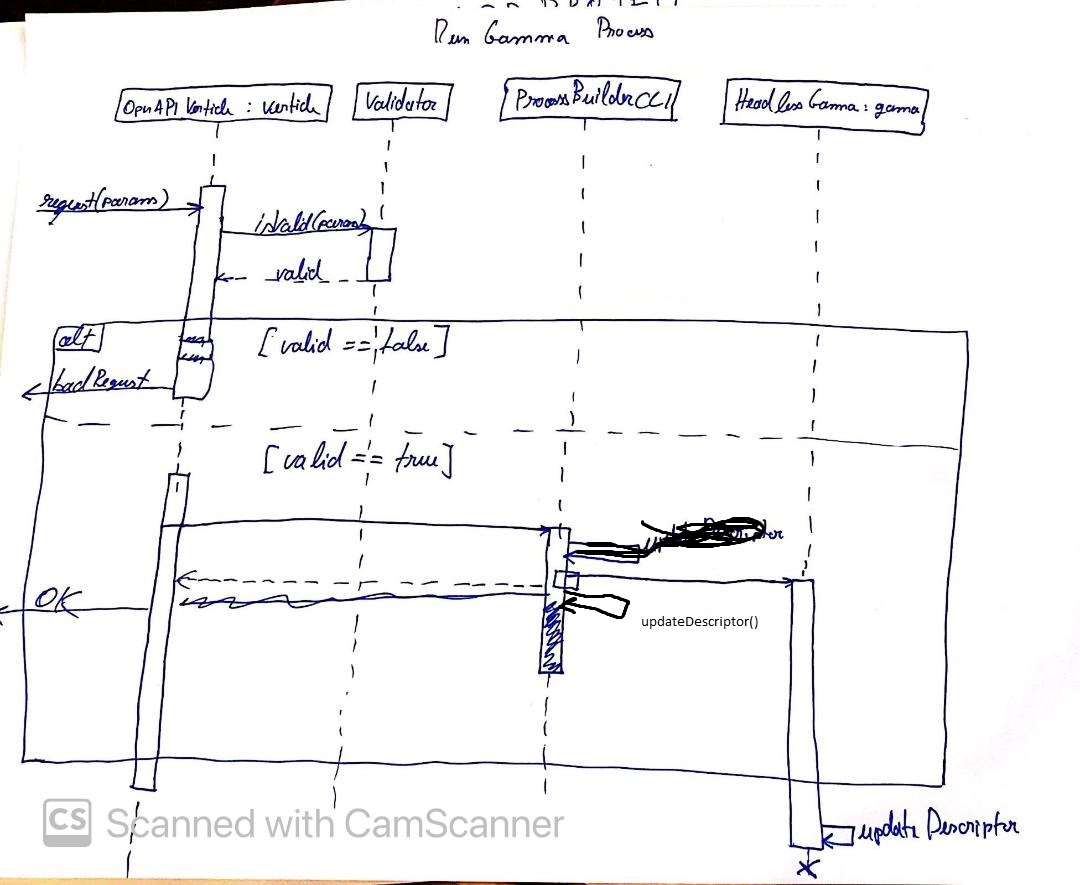
\includegraphics[width=150mm, keepaspectratio]{figures/run_gamma_seq.jpg}
	\caption{Gamma művelet futtatás szekvencia diagram}
	\label{fig:rungamma}
\end{figure}
A gamma műveletek futtatását bemutató szekvencia diagram \aref{fig:rungamma} ábrán tekinthető meg. Ebben az esetben egy PUT HTTP kérés érkezik az \textit{api} endpoint-ra, amit szintén az OpenAPI réteg dolgoz fel kezdetben. A törzsben nem szerepel semmi, viszont az URL-ben utazik a munkatér azonosító, projektnév és futtatni kívánt gamma műveleteket leíró .ggen fájl elérése. Ez a hármas egyedileg meghatározza az erőforrást. A validációs fázis komplexebb ebben az esetben, hiszen ellenőriznünk kell a munkatér-projekt páros létezését és egyediségét, mert egy projekt egyszer szerepelhet egy munkatérben, továbbá azt is meg kell vizsgálni, hogy a projekt, amit ez a páros leír jelenleg használva van-e valamilyen más gamma műveletet futtató headless eclipse által. A Validator döntése alapján, megint két esetet különböztetünk meg, ha valamiért nem felel meg akkor az OpenAPIVerticle a megfelelő hibakóddal és üzenettel visszaszól a kliensnek, hogy nem érvényes a kérés. Ha minden megfelel, akkor a futást átadjuk a ProcessBuilder-nek, ami asszinkron módon elindítja a gamma műveletet futtató headless eclipset. Ezek után egyből frissíti a projektet leíró fájlt, pontosabban, rögzíti az így elindított folyamat operációs rendszer szintű azonosítóját (PID) és beállítja, hogy a projekt futás alatt van. Végezetül átadja a futást a verticle-nek, ami jelzi a kliens felé, hogy a kérés feldolgozása elkezdődött.
A folyamat még nem ér véget, mivel a Gamma dolgozik a háttérben, mikor minden művelet lefutott amit a .ggen fájlban meghatározott a felhasználó, akkor a headless eclipse frissíti a projektet leíró állományt és beállítja, hogy a projekt már nincs futás alatt. További lezáró művelet lehet az értesítés küldés a tárolt email címre, hogy a kért kérés lefutott és az eredmény mostantól lekérhető.


\paragraph{Eredmények lekérése}
\begin{figure}[!ht]
	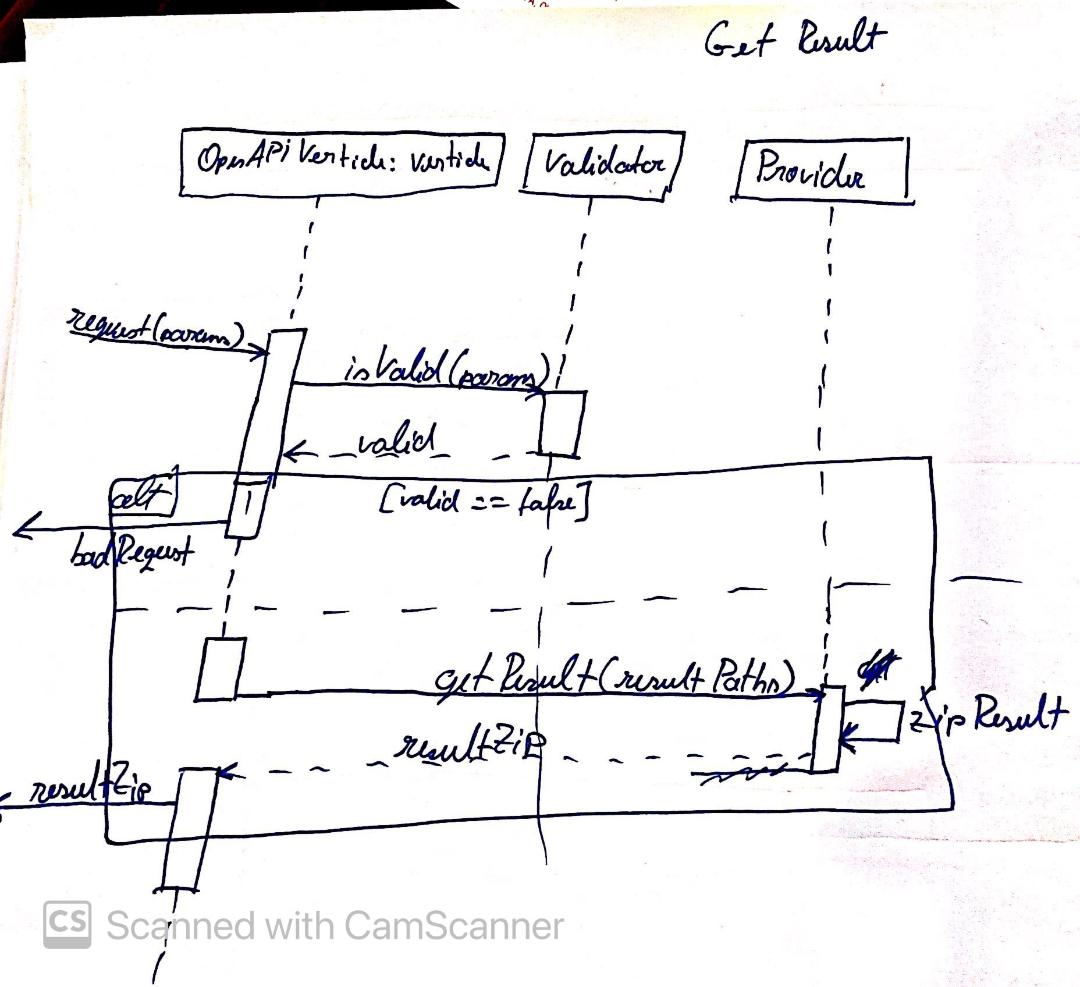
\includegraphics[width=150mm, keepaspectratio]{figures/get_result_seq.jpg}
	\caption{Eredmény lekérés szekvencia diagram}
	\label{fig:getresult}
\end{figure}
A gamma által generált állományok lekérésére szolgáló funkció szekvencia diagramját \aref{fig:getresult} ábra mutatja be. Egy PUT HTTP kérés érkezik a \textit{getresult} endpoint-ra, ennek az URL-jében szerepelnie kell a munkatér azonosítójának és a projektnévnek amiből adatot akarunk lekérni. A kérés törzsében a \textit{resultDirs} attribútum kell szerepeljen, ami egy relatív elérésekből álló lista. A kérés feldolgozása a szokásos módon a verticle-ben kezdődik, ahol a kérésben utazó paraméterek kicsomagolásra kerülnek. A Validator ebben az esetben ugyanazokat ellenőrzi, mint a művelet futtatás folyamat esetén. Ha van futó folyamat a projekten vagy a workspace projekt páros nem megfelelő, akkor beszédes hibaüzenettel válaszolunk a kliensnek. Abban az esetben, ha minden rendben van, akkor a Provider kapja meg  a futási jogot. Itt az elérési listán iterálva összegyűjtjük a kért fájlokat és mappákat majd archiváljuk, az így archivált fájl elérést küldjük vissza a verticle-nek, ami ennek alapján visszaküldi a fájlt.

Első látszatra zavaró lehet, hogy PUT metódust használunk a kérés feldolgozásához, mikor egy GET jobb lehetne és jobban megfelelne a REST szabványnak. Ennek két oka van, az első az, hogy annak ellenére, hogy \textit{getresult}-nak hívjuk az endpoint-ot az erőforrás állapota módosul hiszen a projekten belül generálunk egy archivált fájlt, a másik oka pedig az, hogy a GET kérésnél nem lehet a törzsben semmit sem küldeni, ezt a REST szigorúan megköveteli, nekünk viszont a becsomagolni kívánt állományokat listában kell megadnunk és ezt az URL-ben kényelmetlen lenne kezelni.


%----------------------------------------------------------------------------
\section{Implementáció}
%----------------------------------------------------------------------------

%----------------------------------------------------------------------------
\subsection{Fejlesztés folyamata}
%----------------------------------------------------------------------------


Ebben a fejezetben a fejlesztés során felmerült nehézségeket és érédességeket mutatom be. Az alábbi információk alapvetően mély technikai szintre lemennek így szárazak lehetnek, viszont a témában dolgozóknak hasznos lehet, mert egyedi hibák és jelenségek megoldását vázolom föl.

\paragraph{Eclipse környezettel kapcsolatos érdekességek} Az Eclipse környezetben tapasztalt fejlesztők tudják, hogy bizonyos dolgok nem triviálisak a fejlesztés során és olyan specifikus problémák merülhetnek fel, amelyekre nagyon elrejtett internetes fórumokon lehet választ kapni. Az alábbi jelenségek és problémák a \textit{Headless Gamma} komponens fejlesztése alatt merültek föl

Az eclipse plug-in fejlesztés és termék export konfiguráció során számos függősségi problémával szembesültem. A legelső érdekesség ami felmerült, az volt, hogy az Eclipse a \textit{product} konfigurációban meghatározott plug-in függőségek verzióját automatikusan felülírta a környezetbe telepített legfrissebb verzióval. Ezen plug-in-ek listáját az Eclipse IDE-n belül a \textit{Target Platform}-on lehet megtekinteni és szerkeszteni. Ilyen problémás függőségek voltak a \textit{batik.css} és \textit{batik.util} plug-in-ek. A Target Platform szerkesztésével ezt a problémát orvosolni lehet, csupán ki kell vegyük vagy hozzá kell adjuk azt a verziót amire szükségünk van és győződjünk meg, hogy az adott plug-in-ből csak egy verziót aktív.

A product konfigurációban a \textit{Content} fülön tudjuk meghatározni milyen plug-in-ekből álljon a termékünk, az IDE-ben lehetőség van arra, hogy megadjuk a fejlesztett alkalmazásunkat és rányomva az \textit{Add Requiered} gombra az IDE automatikusan beállítja a termékünk összes függőségét. Ennek ellenére az osgi.extender olyan plug-in-eket igényel, amelyek az OSGi helyes működéséhez szükségesek de nem importálja be automatikusan. A szükséges modulok:
\begin{lstlisting}[language=]
org.apache.felix.scr
org.eclipse.equinox.event
org.eclipse.compare.core
org.eclipse.fx.osgi
org.eclipse.team.core
\end{lstlisting}

Olyan jelenség is előjött, ahol a függőségi fában egy plug-in kétszer szerepelt viszont különböző verzióval, ezt az OSGi szabvány engedi de az Eclipse, az első jelenségben leírtak alapján, folyamatosan felülírta az elavultabb verziót. A probléma elképzelésében segít  \aref{fig:depend} ábra. Erre a megoldás az, hogy a fában felfele haladva megvizsgáljuk, hogy milyen verziókat tudunk frissíteni a Target Platformon úgy, hogy a működést megtartsuk de az elavult verziójú plug-in-t frissíteni tudjuk. Alapvetően egyszerű feladatnak tűnik, viszont a rendszer közel 250 függőséggel rendelkezik.

\begin{figure}[t]
	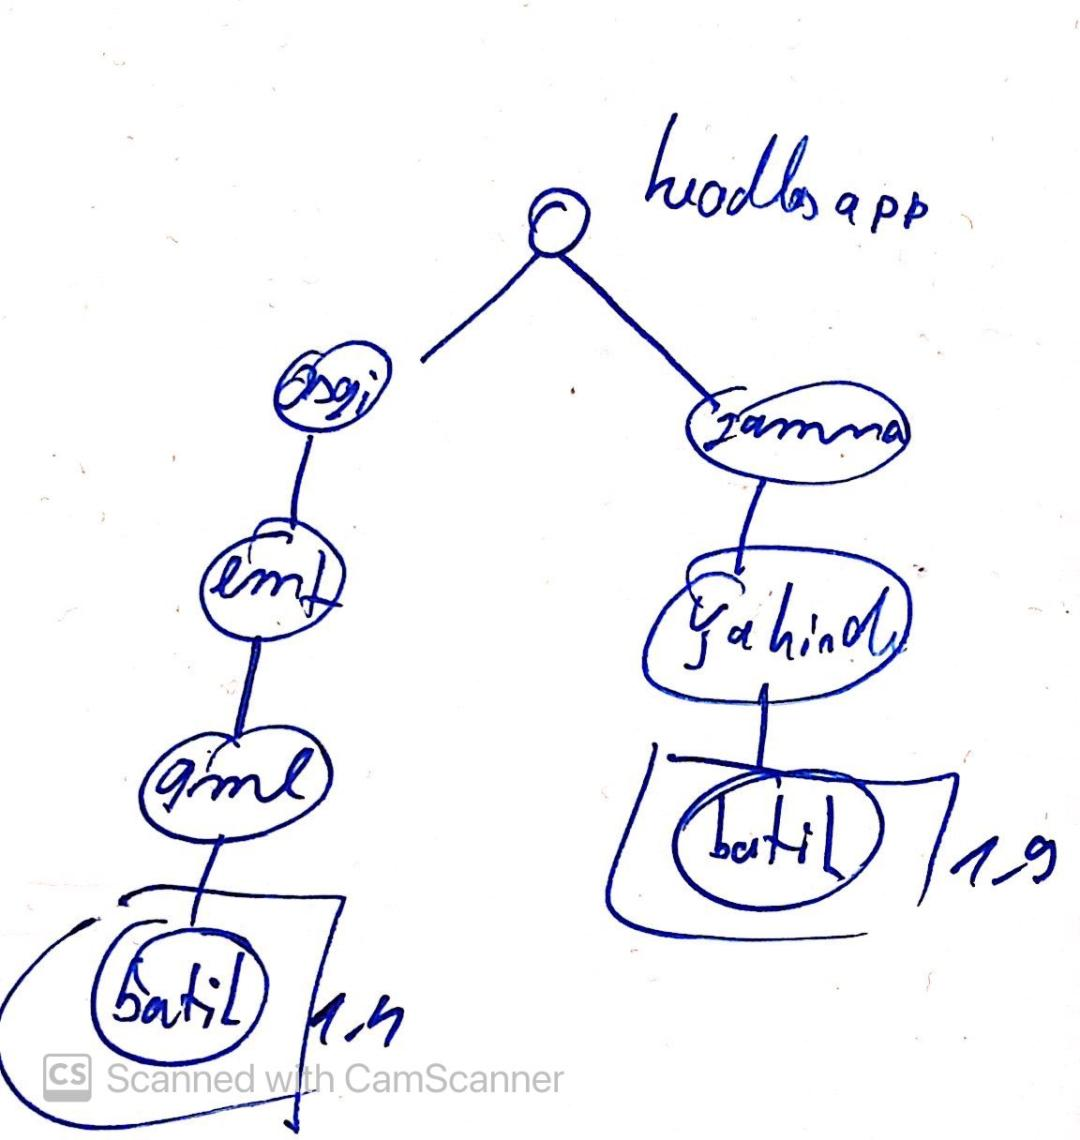
\includegraphics[width=150mm, keepaspectratio]{figures/depend.jpg}
	\caption{Egyszerűsített függőségi fa}
	\label{fig:depend}
\end{figure}

A termék export felületen meg kell határozni, hogy az egyes Eclipse modulok milyen sorrendbe induljanak el, a mi esetünkbe az alábbi indulási szintek meghatározása volt fontos:
\begin{lstlisting}[language=XML]
<configurations>
	<plugin id="org.apache.felix.scr" autoStart="true" startLevel="2" />
	<plugin id="org.eclipse.core.runtime" autoStart="true" startLevel="0" />
	<plugin id="org.eclipse.equinox.common" autoStart="true" startLevel="2" />
	<plugin id="org.eclipse.equinox.event" autoStart="true" startLevel="2" />
	<plugin id="org.eclipse.equinox.simpleconfigurator" autoStart="true" startLevel="1" />
</configurations>
\end{lstlisting}
Ez a konfiguráció részlet a termék leírás XML fájlból van másolva, az IDE-ben a \textit{Configuration} fülön lehet mindezt beállítani.

Egy termék konfiguráció futtatására két lehetőségünk van, az első, hogy exportáljuk (headless eclipse) majd parancssorból meghívjuk és átadjuk az argumentumokat vagy az IDE-ből elindítjuk. Az utóbbi tesztelés folyamán nagyon hasznos tud lenni. Ha IDE-ből futtatjuk akkor is van lehetőségünk argumentumokat átadni, erre szintén a termék konfigurációban van lehetőség, pontosabban a \textit{Launching} fülön. Arra viszont érdemes odafigyelni, hogy ezt a tesztelés után ne hagyjuk ott, mivel az export konstans argumentumoknak értelmezi és minden headless módban indulásnál átadja önmagának. A mi esetünkbe ez hatványozottan fontos, mivel az átadott argumentumok minden esetben mások a munkatér és projektek számossága miatt.

Minden függőség lehet opcionális vagy kötelező az opcionálisakat csak abban az esetben tölti be a headless eclipse mikor éppen szüksége van rá. A rendszerünknek a \textit{jdt} plug-in család több komponensére is szüksége van viszont ezek a függőségi fában levő szülőjükön a \textit{xtext.ui} plug-in-en csupán opcionálisként vannak megjelölve és egy mai napig nem tisztázott ok miatt nem töltődtek be. A problémát azzal lehet orvosolni, hogy készítünk az xtext.ui plug-in-ből egy saját példányt, amin a függőségi beállításokat átírjuk opcionálisról kötelezőre. Ez sajnos nehezíti a rendszer tovább fejlesztését és a telepítési folyamat is komplexebbé válik.

Egy kulcsfontosságú probléma az volt, hogy az Xtext\footnote{Xtext-ről többet: \url{https://www.eclipse.org/Xtext/}} modult eddig nem tudtuk injektálni a headless eclipse-be. Erre az alábbi kódrészlet ad megoldást:
\begin{lstlisting}[language=Java]
 	Injector injector = new StatechartLanguageStandaloneSetupGenerated()
 							.createInjectorAndDoEMFRegistration();
 	XtextResourceSet resourceSet = injector.getInstance(XtextResourceSet.class);
\end{lstlisting}
A fent definiált \textit{resourceSet}-ről tudjuk majd a headless eclipse-nek argumentumban átadott fájlt elérni.

Minden Gamma nyelv interpretálóját egyedileg meg kellet hívni az alkalmazás indulási pillanataiban:

\begin{lstlisting}[language=Java]
//Alkalmazás belépési pontja
 @Override
public Object start(final IApplicationContext context) throws Exception {
	ExpressionLanguageStandaloneSetup.doSetup();
	ActionLanguageStandaloneSetup.doSetup();
	StatechartLanguageStandaloneSetup.doSetup();
	TraceLanguageStandaloneSetup.doSetup();
	PropertyLanguageStandaloneSetup.doSetup();        
	GenModelStandaloneSetup.doSetup();
	.
	.
	.
}
\end{lstlisting}

\paragraph{OpenAPI REST webszerver} Olyan fejlesztői megoldásokat mutatok be, amelyek az OpenAPI és Vert.x használata által nagyon egyszerűen megvalósíthatóak voltak. Ehhez tekintsük át \aref{fig:endpoint_example} ábrát amely az \textit{addproject} endpoint specifikációját tartalmazza.

A Vert.x, mint említettem támogatja az OpenAPI REST specifikáció integrációját, így kódból az alábbi módon tudjuk elérni a fájlban definiált \textit{endpointot} (gamma-wrapper.yaml), amit majd regisztrálunk a webszerverünkbe:
\begin{lstlisting}[language=Java]
@Override
public void start(Future<Void> future) {
        OpenAPI3RouterFactory.create(this.vertx, "gamma-wrapper.yaml", ar ->
		{
               	OpenAPI3RouterFactory routerFactory = ar.result();
                routerFactory.addHandlerByOperationId("addProject", routingContext -> {	... });
				...	
		});
}
\end{lstlisting}
A fenti kódrészletben már nagyon egyszerűen tudjuk a kérésben utazó paramétereket Java objektummá átalakítani.A példában fájlok feldolgozását is el kell végezzük, ezt a Vert.x a fenti \textit{routingContext} objektumon már eltárolja és egy egyszerű \textit{routingContext.fileUploads()} hívással már \textit{File} objektumok listáját kapjuk vissza.


Bizonyos validációs feladatokat is elvégez helyettünk az OpenAPI definíció alapján a Vert.x, \aref{fig:endpoint_example} ábrán látható, hogy meghatározzuk a munkatér(workspace) szintaktikáját, ha ettől eltérő, más formátumú karakterlánc szerepel a kérésben akkor automatikusan küldődik egy válasz a klienshez, hogy nem megfelelő a kérése.



\begin{figure}[!ht]
	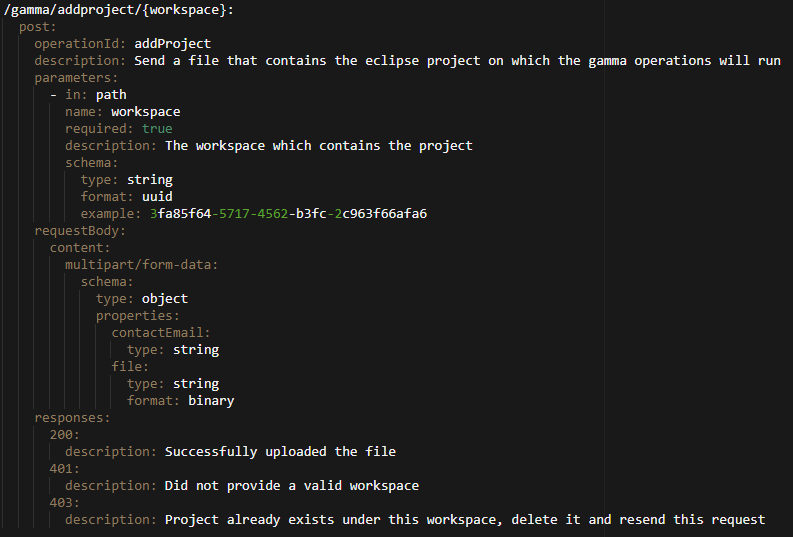
\includegraphics[width=150mm, keepaspectratio]{figures/endpoint_example.png}
	\caption{Endpoint példa}
	\label{fig:endpoint_example}
\end{figure}

\paragraph{ProcessBuilder fejlesztés} Alapvetően a webszerver java 8 alapokon lett megvalósítva, majd kiderült, hogy a java 9 hasznos, új frissítéseket tartalmaz a \textit{java.lang.ProcessBuilder} komponensén. Számunkra ez azért fontos, mert bevezetésre került a \textit{pid} (process id) lekérése az éppen indított folyamatról. Ezt az azonosítót feltudjuk használni, hogy egy Gamma műveleteket feldolgozó folyamatot leállítsunk, ha úgy gondoljuk, hogy túl sok ideig fut.
Nagyon fontos megjegyezni azt, hogy ha folyamatot indítunk a \textit{java.lang.ProcessBuilder} segítségével és ez több ideig fut, akkor a logolási eredményét kötelezően át kell irányítsuk fájlba vagy konzolba. Ennek hiányában a folyamatunk beakad. A rendszerünk a folyamatot indító konténerre leörökölteti a logolás feladatát. A HeadlessGamma elindítására szolgáló kódrészlet:

\begin{lstlisting}[language=Java]
	ProcessBuilder pb = new ProcessBuilder(commandToBeExecuted); // ProcessBuilder inicializálás, commandToBeExecuted a futtatni kivánt parancs karakterláncát tartalmazza
	pb.redirectErrorStream(true);
	pb.inheritIO(); // Logolás öröklés
	long pib =  pb.start().pid(); // Folyamat azonosító lekérése
}
\end{lstlisting}


%----------------------------------------------------------------------------
\subsection{Rendszer szoftverkomponensei}
%----------------------------------------------------------------------------

A rendszer struktúrájából kiindulva, ezt \aref{fig:structure} ábrán lehet megtekinteni, a rendszer szoftver szintű felépítése három komponensből tevődik össze, ezek vizuális reprezentációját \aref{fig:software_components} ábra mutatja be.

\begin{figure}[t]
	\centering
	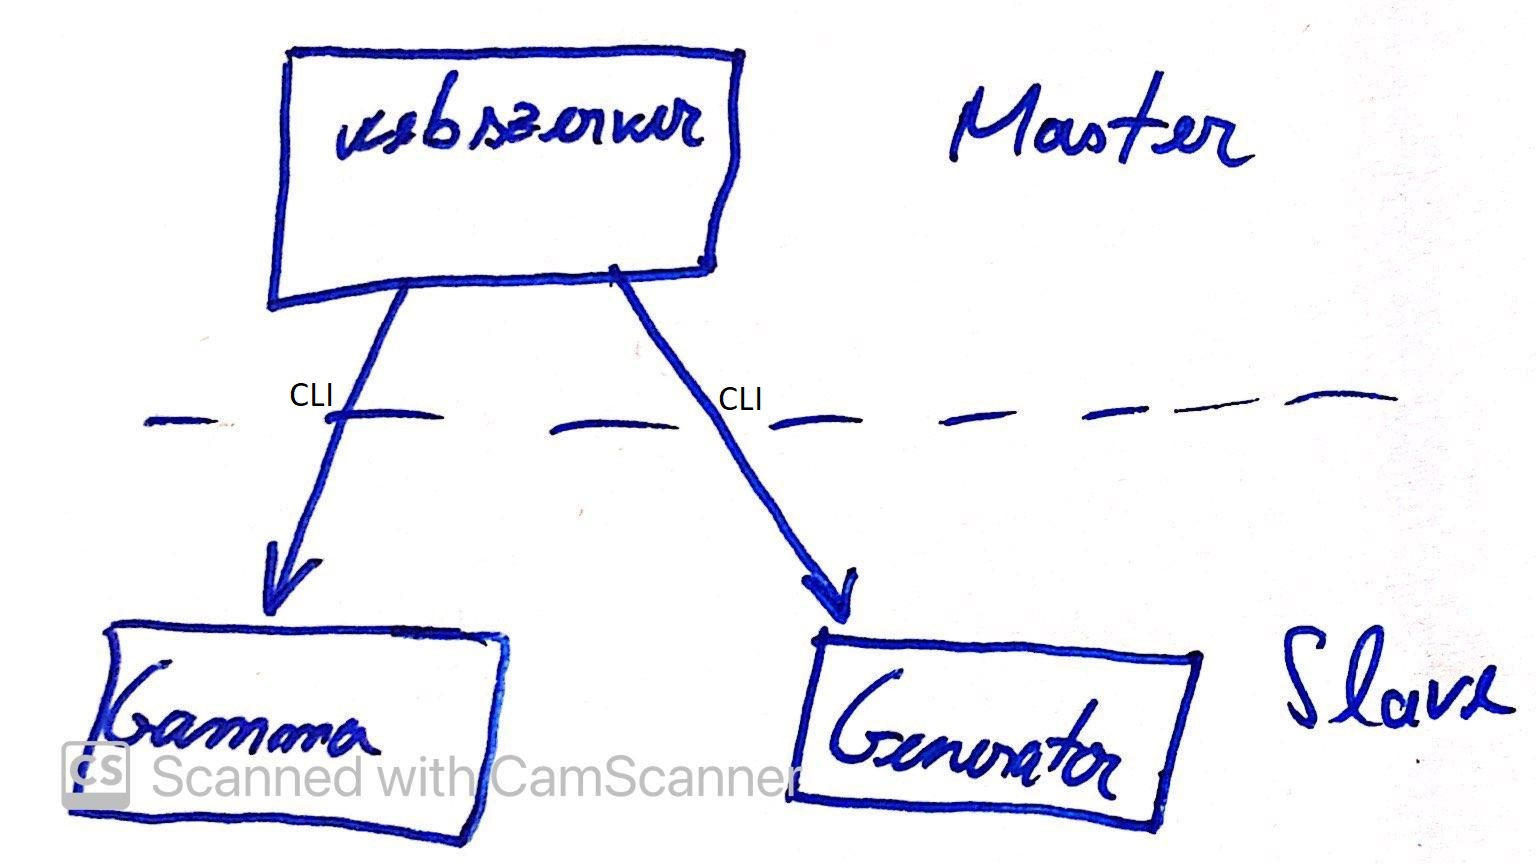
\includegraphics[width=75mm, keepaspectratio]{figures/software_components.jpg}
	\caption{Szoftver komponensek}
	\label{fig:software_components}
\end{figure}

A Webszerver tartalmazza az összes olyan komponenst, amely a webes kérések értelmezését és átalakítását végzik, itt található az OpenAPI definíció. Önmagában egy Maven\footnote{Maven-ről többet: \url{https://maven.apache.org/}} alapú InteliJ IDEA-ban fejlesztett alkalmazás. A Gamma és a Generator pedig az eddigiekben már többször említett két headless eclipse alkalmazás. A webszerver egy master szerepet tölt be a rendszerünkbe, mivel ö koordinálja a másik kettő működését.

% !TeX spellcheck = hu_HU
% !TeX encoding = UTF-8
% !TeX program = xelatex
%----------------------------------------------------------------------------
\chapter{A \LaTeX-sablon használata}
%----------------------------------------------------------------------------

Ebben a fejezetben röviden, implicit módon bemutatjuk a sablon használatának módját, ami azt jelenti, hogy sablon használata ennek a dokumentumnak a forráskódját tanulmányozva válik teljesen világossá. Amennyiben a szoftver-keretrendszer telepítve van, a sablon alkalmazása és a dolgozat szerkesztése \LaTeX-ben a sablon segítségével tapasztalataink szerint jóval hatékonyabb, mint egy WYSWYG (\emph{What You See is What You Get}) típusú szövegszerkesztő esetén (pl. Microsoft Word, OpenOffice).

%----------------------------------------------------------------------------
\section{Címkék és hivatkozások}
%----------------------------------------------------------------------------
A \LaTeX~dokumentumban címkéket (\verb+\label+) rendelhetünk ábrákhoz, táblázatokhoz, fejezetekhez, listákhoz, képletekhez stb. Ezekre a dokumentum bármely részében hivatkozhatunk, a hivatkozások automatikusan feloldásra kerülnek.

A sablonban makrókat definiáltunk a hivatkozások megkönnyítéséhez. Ennek megfelelően minden ábra (\emph{figure}) címkéje \verb+fig:+ kulcsszóval kezdődik, míg minden táblázat (\emph{table}), képlet (\emph{equation}), fejezet (\emph{section}) és lista (\emph{listing}) rendre a \verb+tab:+, \verb+eq:+, \verb+sec:+ és \verb+lst:+ kulcsszóval kezdődik, és a kulcsszavak után tetszőlegesen választott címke használható. Ha ezt a konvenciót betartjuk, akkor az előbbi objektumok számára rendre a \verb+\figref+, \verb+\tabref+, \verb+\eqref+, \verb+\sectref+ és \verb+\listref+ makrókkal hivatkozhatunk. A makrók paramétere a címke, amelyre hivatkozunk (a kulcsszó nélkül). Az összes említett hivatkozástípus, beleértve az \verb+\url+ kulcsszóval bevezetett web-hivatkozásokat is a  \verb+hyperref+\footnote{Segítségével a dokumentumban megjelenő hivatkozások nem csak dinamikussá válnak, de színezhetők is, bővebbet erről a csomag dokumentációjában találunk. Ez egyúttal egy példa lábjegyzet írására.} csomagnak köszönhetően aktívak a legtöbb PDF-nézegetőben, rájuk kattintva a dokumentum megfelelő oldalára ugrik a PDF-néző vagy a megfelelő linket megnyitja az alapértelmezett böngészővel. A \verb+hyperref+ csomag a kimeneti PDF-dokumentumba könyvjelzőket is készít a tartalomjegyzékből. Ez egy szintén aktív tartalomjegyzék, amelynek elemeire kattintva a nézegető behozza a kiválasztott fejezetet.

%----------------------------------------------------------------------------
\section{Ábrák és táblázatok}
%----------------------------------------------------------------------------
Használjunk vektorgrafikus ábrákat, ha van rá módunk. PDFLaTeX használata esetén PDF formátumú ábrákat lehet beilleszteni könnyen, az EPS (PostScript) vektorgrafikus képformátum beillesztését a PDFLaTeX közvetlenül nem támogatja (de lehet konvertálni, lásd később). Ha vektorgrafikus formában nem áll rendelkezésünkre az ábra, akkor a  veszteségmentes PNG, valamint a veszteséges JPEG formátumban érdemes elmenteni.  Figyeljünk arra, hogy ilyenkor a képek felbontása elég nagy legyen ahhoz, hogy nyomtatásban is megfelelő minőséget nyújtson (legalább 300 dpi javasolt). A dokumentumban felhasznált képfájlokat a dokumentum forrása mellett érdemes tartani, archiválni, mivel ezek hiányában a dokumentum nem fordul újra. Ha lehet, a vektorgrafikus képeket vektorgrafikus formátumban is érdemes elmenteni az újrafelhasználhatóság (az átszerkeszthetőség) érdekében.

Kapcsolási rajzok legtöbbször kimásolhatók egy vektorgrafikus programba (pl. CorelDraw) és onnan nagyobb felbontással raszterizálva kimenthatők PNG formátumban. Ugyanakkor kiváló ábrák készíthetők Microsoft Visio vagy hasonló program használatával is: Visio-ból az ábrák közvetlenül PDF-be is menthetők.

Lehetőségeink Matlab ábrák esetén:
\begin{itemize}
	\item Képernyőlopás (\emph{screenshot}) is elfogadható minőségű lehet a dokumentumban, de általában jobb felbontást is el lehet érni más módszerrel.
	\item A Matlab ábrát a \verb+File/Save As+ opcióval lementhetjük PNG formátumban (ugyanaz itt is érvényes, mint korábban, ezért nem javasoljuk).
	\item A Matlab ábrát az \verb+Edit/Copy figure+ opcióval kimásolhatjuk egy vektorgrafikus programba is és onnan nagyobb felbontással raszterizálva kimenthatjük PNG formátumban (nem javasolt).
	\item Javasolt megoldás: az ábrát a \verb+File/Save As+ opcióval EPS \emph{vektorgrafikus} formátumban elmentjük, PDF-be konvertálva beillesztjük a dolgozatba.
\end{itemize}
Az EPS kép az \verb+epstopdf+ programmal\footnote{a korábban említett \LaTeX-disztribúciókban megtalálható} konvertálható PDF formátumba. Célszerű egy batch-fájlt készíteni az összes EPS ábra lefordítására az alábbi módon (ez Windows alatt működik).
\begin{lstlisting}[language=]
@echo off
for %%j in (*.eps) do (
  echo converting file "%%j"
  epstopdf "%%j"
)
echo done .
\end{lstlisting}

Egy ilyen parancsfájlt (\verb+convert.cmd+) elhelyeztük a sablon \verb+figures\eps+ könyvtárába, így a felhasználónak csak annyi a dolga, hogy a \verb+figures\eps+ könyvtárba kimenti az EPS formátumú vektorgrafikus képet, majd lefuttatja a \verb+convert.cmd+ parancsfájlt, ami PDF-be konvertálja az EPS fájlt.

Ezek után a PDF-ábrát ugyanúgy lehet a dokumentumba beilleszteni, mint a PNG-t vagy a JPEG-et. A megoldás előnye, hogy a lefordított dokumentumban is vektorgrafikusan tárolódik az ábra, így a mérete jóval kisebb, mintha raszterizáltuk volna beillesztés előtt. Ez a módszer minden -- az EPS formátumot ismerő -- vektorgrafikus program (pl. CorelDraw) esetén is használható.

A képek beillesztésére \az+\refstruc{sec:LatexTools}ben mutattunk be példát (\refstruc{fig:TeXstudio}). Az előző mondatban egyúttal az automatikusan feloldódó ábrahivatkozásra is láthatunk példát. Több képfájlt is beilleszthetünk egyetlen ábrába. Az egyes képek közötti horizontális és vertikális margót metrikusan szabályozhatjuk (\refstruc{fig:HVSpaces}). Az ábrák elhelyezését számtalan tipográfiai szabály egyidejű teljesítésével a fordító maga végzi, a dokumentum írója csak preferenciáit jelezheti a fordító felé (olykor ez bosszúságot is okozhat, ilyenkor pl. a kép méretével lehet játszani).

\begin{figure}[!ht]
	\centering
	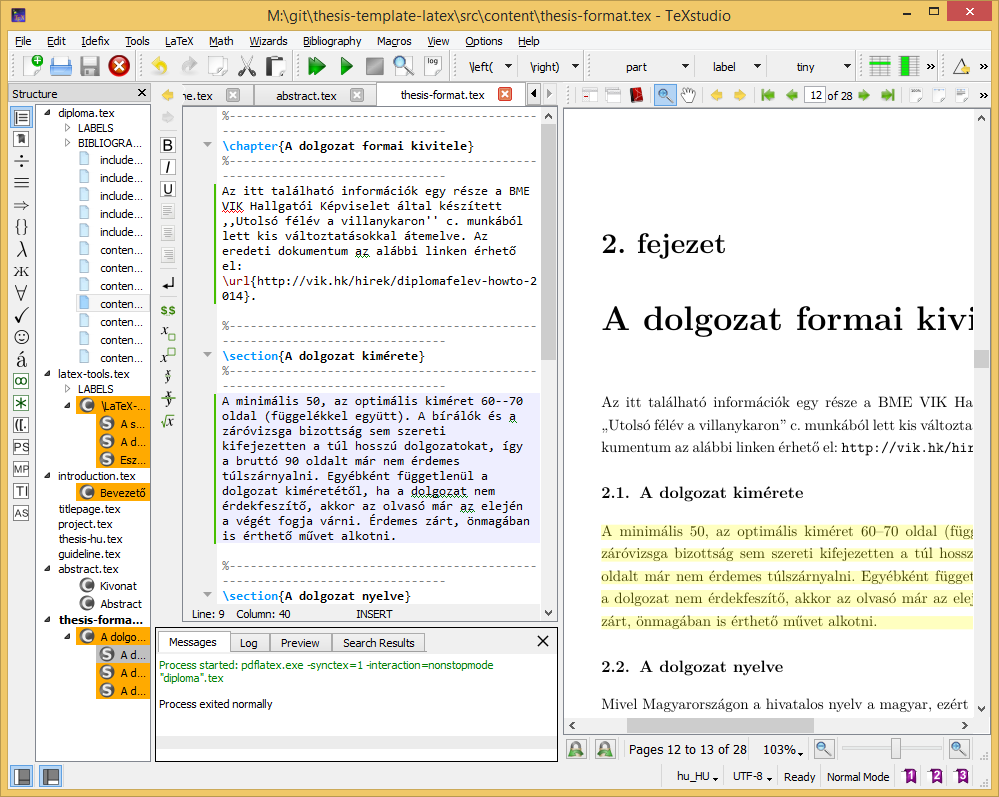
\includegraphics[width=67mm, keepaspectratio]{figures/TeXstudio.png}\hspace{1cm}
	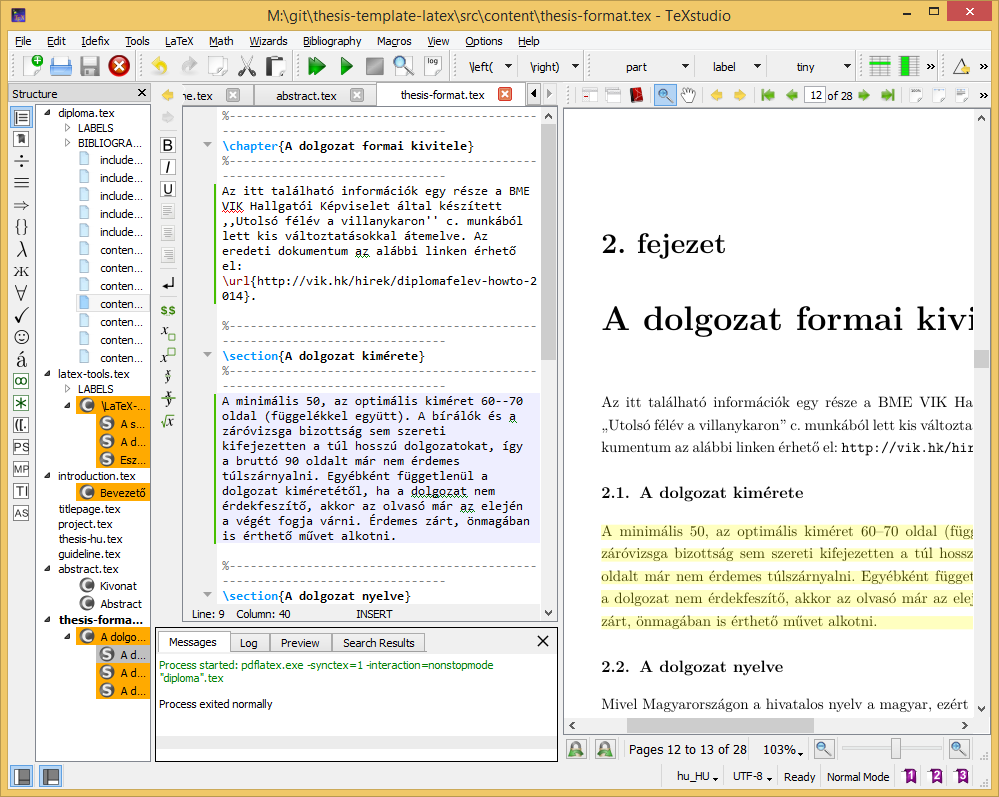
\includegraphics[width=67mm, keepaspectratio]{figures/TeXstudio.png}\\\vspace{5mm}
	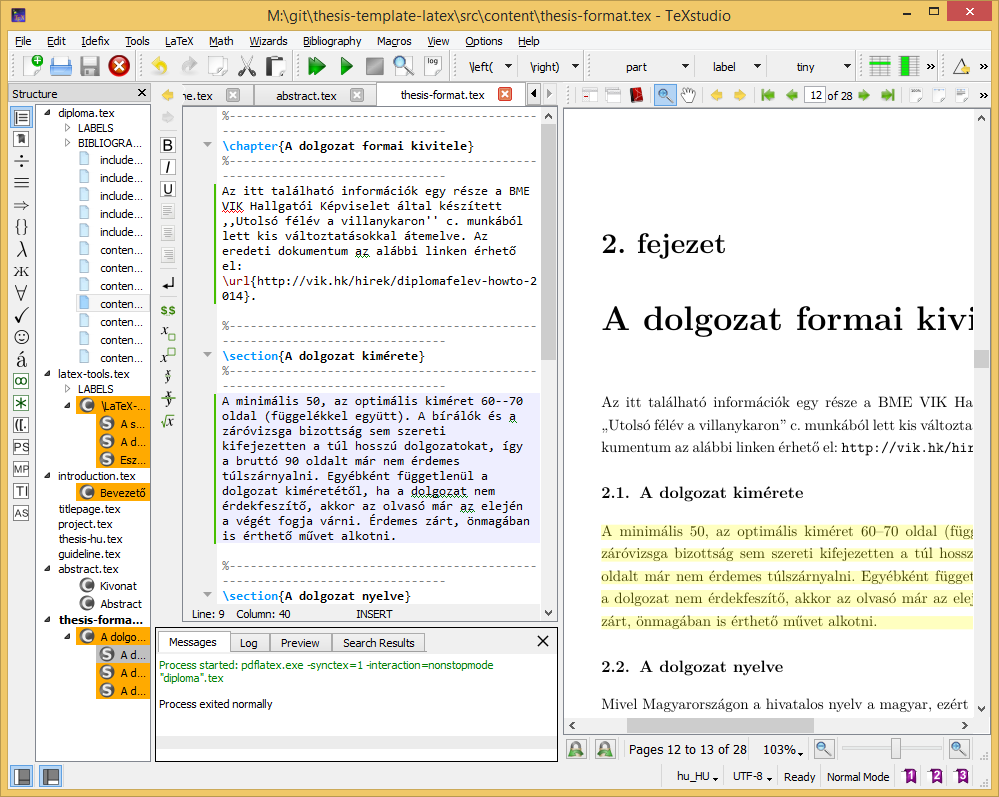
\includegraphics[width=67mm, keepaspectratio]{figures/TeXstudio.png}\hspace{1cm}
	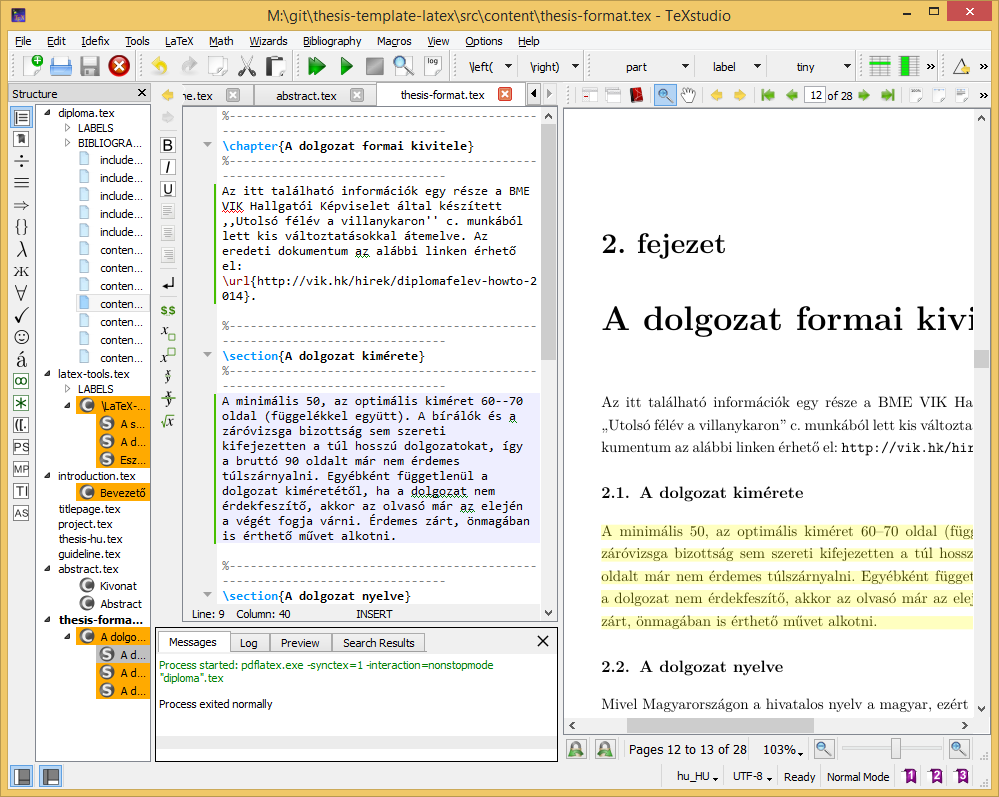
\includegraphics[width=67mm, keepaspectratio]{figures/TeXstudio.png}
	\caption{Több képfájl beillesztése esetén térközöket is érdemes használni.}
	\label{fig:HVSpaces}
\end{figure}

A táblázatok használatára \aref{tab:TabularExample}~táblázat mutat példát. A táblázatok formázásához hasznos tanácsokat találunk a \verb+booktabs+ csomag dokumentációjában.

\begin{table}[ht]
	\footnotesize
	\centering
	\begin{tabular}{ l c c }
		\toprule
		Órajel & Frekvencia & Cél pin \\
		\midrule
		CLKA & 100 MHz & FPGA CLK0\\
		CLKB & 48 MHz  & FPGA CLK1\\
		CLKC & 20 MHz  & Processzor\\
		CLKD & 25 MHz  & Ethernet chip \\
		CLKE & 72 MHz  & FPGA CLK2\\
		XBUF & 20 MHz  & FPGA CLK3\\
		\bottomrule
	\end{tabular}
	\caption{Az órajel-generátor chip órajel-kimenetei.}
	\label{tab:TabularExample}
\end{table}


%----------------------------------------------------------------------------
\section{Felsorolások és listák}
%----------------------------------------------------------------------------
Számozatlan felsorolásra mutat példát a jelenlegi bekezdés:
\begin{itemize}
	\item \emph{első bajusz:} ide lehetne írni az első elem kifejését,
	\item \emph{második bajusz:} ide lehetne írni a második elem kifejését,
	\item \emph{ez meg egy szakáll:} ide lehetne írni a harmadik elem kifejését.
\end{itemize}

Számozott felsorolást is készíthetünk az alábbi módon:
\begin{enumerate}
	\item \emph{első bajusz:} ide lehetne írni az első elem kifejését, és ez a kifejtés így néz ki, ha több sorosra sikeredik,
	\item \emph{második bajusz:} ide lehetne írni a második elem kifejését,
	\item \emph{ez meg egy szakáll:} ide lehetne írni a harmadik elem kifejését.
\end{enumerate}
A felsorolásokban sorok végén vessző, az utolsó sor végén pedig pont a szokásos írásjel. Ez alól kivételt képezhet, ha az egyes elemek több teljes mondatot tartalmaznak.

Listákban a dolgozat szövegétől elkülönítendő kódrészleteket, programsorokat, pszeudo-kódokat jeleníthetünk meg (\ref{lst:Example}.~kódrészlet).
\begin{lstlisting}[language=tex,caption=A fenti számozott felsorolás \LaTeX-forráskódja,label=lst:Example]
\begin{enumerate}
	\item \emph{els(*@ő@*) bajusz:} ide lehetne írni az els(*@ő@*) elem kifejését,
	és ez a kifejtés így néz ki, ha több sorosra sikeredik,
	\item \emph{második bajusz:} ide lehetne írni a második elem kifejését,
	\item \emph{ez meg egy szakáll:} ide lehetne írni a harmadik elem kifejését.
\end{enumerate}
\end{lstlisting}
A lista keretét, háttérszínét, egész stílusát megválaszthatjuk. Ráadásul különféle programnyelveket és a nyelveken belül kulcsszavakat is definiálhatunk, ha szükséges. Erről bővebbet a \verb+listings+ csomag hivatalos leírásában találhatunk.

%----------------------------------------------------------------------------
\section{Képletek}
%----------------------------------------------------------------------------
Ha egy formula nem túlságosan hosszú, és nem akarjuk hivatkozni a szövegből, mint például a $e^{i\pi}+1=0$ képlet, \emph{szövegközi képletként} szokás leírni. Csak, hogy másik példát is lássunk, az $U_i=-d\Phi/dt$ Faraday-törvény a $\rot E=-\frac{dB}{dt}$ differenciális alakban adott Maxwell-egyenlet felületre vett integráljából vezethető le. Látható, hogy a \LaTeX-fordító a sorközöket betartja, így a szöveg szedése esztétikus marad szövegközi képletek használata esetén is.

Képletek esetén az általános konvenció, hogy a kisbetűk skalárt, a kis félkövér betűk ($\mathbf{v}$) oszlopvektort -- és ennek megfelelően $\mathbf{v}^T$ sorvektort -- a kapitális félkövér betűk ($\mathbf{V}$) mátrixot jelölnek. Ha ettől el szeretnénk térni, akkor az alkalmazni kívánt jelölésmódot célszerű külön alfejezetben definiálni. Ennek megfelelően, amennyiben $\mathbf{y}$ jelöli a mérések vektorát, $\mathbf{\vartheta}$ a paraméterek vektorát és $\hat{\mathbf{y}}=\mathbf{X}\vartheta$ a paraméterekben lineáris modellt, akkor a \emph{Least-Squares} értelemben optimális paraméterbecslő $\hat{\mathbf{\vartheta}}_{LS}=(\mathbf{X}^T\mathbf{X})^{-1}\mathbf{X}^T\mathbf{y}$ lesz.

Emellett kiemelt, sorszámozott képleteket is megadhatunk, ennél az \verb+equation+ és a \verb+eqnarray+ környezetek helyett a korszerűbb \verb+align+ környezet alkalmazását javasoljuk (több okból, különféle problémák elkerülése végett, amelyekre most nem térünk ki). Tehát
\begin{align}
\dot{\mathbf{x}}&=\mathbf{A}\mathbf{x}+\mathbf{B}\mathbf{u},\\
\mathbf{y}&=\mathbf{C}\mathbf{x},
\end{align}
ahol $\mathbf{x}$ az állapotvektor, $\mathbf{y}$ a mérések vektora és $\mathbf{A}$, $\mathbf{B}$ és $\mathbf{C}$ a rendszert leíró paramétermátrixok. Figyeljük meg, hogy a két egyenletben az egyenlőségjelek egymáshoz igazítva jelennek meg, mivel a mindkettőt az \& karakter előzi meg a kódban. Lehetőség van számozatlan kiemelt képlet használatára is, például
\begin{align}
\dot{\mathbf{x}}&=\mathbf{A}\mathbf{x}+\mathbf{B}\mathbf{u},\nonumber\\
\mathbf{y}&=\mathbf{C}\mathbf{x}\nonumber.
\end{align}
Mátrixok felírására az $\mathbf{A}\mathbf{x}=\mathbf{b}$ inhomogén lineáris egyenlet részletes kifejtésével mutatunk példát:
\begin{align}
\begin{bmatrix}
a_{11} & a_{12} & \dots & a_{1n}\\
a_{21} & a_{22} & \dots & a_{2n}\\
\vdots & \vdots & \ddots & \vdots\\
a_{m1} & a_{m2} & \dots & a_{mn}
\end{bmatrix}
\begin{pmatrix}x_1\\x_2\\\vdots\\x_n\end{pmatrix}=
\begin{pmatrix}b_1\\b_2\\\vdots\\b_m\end{pmatrix}.
\end{align}
A \verb+\frac+ utasítás hatékonyságát egy általános másodfokú tag átviteli függvényén keresztül mutatjuk be, azaz
\begin{align}
W(s)=\frac{A}{1+2T\xi s+s^2T^2}.
\end{align}
A matematikai mód minden szimbólumának és képességének a bemutatására természetesen itt nincs lehetőség, de gyors referenciaként hatékonyan használhatók a következő linkek:\\
\indent\url{http://www.artofproblemsolving.com/LaTeX/AoPS_L_GuideSym.php},\\
\indent\url{http://www.ctan.org/tex-archive/info/symbols/comprehensive/symbols-a4.pdf},\\
\indent\url{ftp://ftp.ams.org/pub/tex/doc/amsmath/short-math-guide.pdf}.\\
Ez pedig itt egy magyarázat, hogy miért érdemes \verb+align+ környezetet használni:\\
\indent\url{http://texblog.net/latex-archive/maths/eqnarray-align-environment/}.

%----------------------------------------------------------------------------
\section{Irodalmi hivatkozások}
\label{sec:HowtoReference}
%----------------------------------------------------------------------------
Egy \LaTeX~dokumentumban az irodalmi hivatkozások definíciójának két módja van. Az egyik a \verb+\thebibliograhy+ környezet használata a dokumentum végén, az \verb+\end{document}+ lezárás előtt.
\begin{lstlisting}[language=tex]
\begin{thebibliography}{9}

\bibitem{Lamport94} Leslie Lamport, \emph{\LaTeX: A Document Preparation System}.
Addison Wesley, Massachusetts, 2nd Edition, 1994.

\end{thebibliography}
\end{lstlisting}

Ezek után a dokumentumban a \verb+\cite{Lamport94}+ utasítással hivatkozhatunk a forrásra. A fenti megadás viszonylag kötetlen, a szerző maga formázza az irodalomjegyzéket (ami gyakran inkonzisztens eredményhez vezet).

Egy sokkal professzionálisabb módszer a BiB\TeX{} használata, ezért ez a sablon is ezt támogatja. Ebben az esetben egy külön szöveges adatbázisban definiáljuk a forrásmunkákat, és egy külön stílusfájl határozza meg az irodalomjegyzék kinézetét. Ez, összhangban azzal, hogy külön formátumkonvenció határozza meg a folyóirat-, a könyv-, a konferenciacikk- stb. hivatkozások kinézetét az irodalomjegyzékben (a sablon használata esetén ezzel nem is kell foglalkoznia a hallgatónak, de az eredményt célszerű ellenőrizni). felhasznált hivatkozások adatbázisa egy \verb+.bib+ kiterjesztésű szöveges fájl, amelynek szerkezetét a \Aref{lst:Bibtex} kódrészlet demonstrálja. A forrásmunkák bevitelekor a sor végi vesszők külön figyelmet igényelnek, mert hiányuk a BiB\TeX-fordító hibaüzenetét eredményezi. A forrásmunkákat típus szerinti kulcsszó vezeti be (\verb+@book+ könyv, \verb+@inproceedings+ konferenciakiadványban megjelent cikk, \verb+@article+ folyóiratban megjelent cikk, \verb+@techreport+ valamelyik egyetem gondozásában megjelent műszaki tanulmány, \verb+@manual+ műszaki dokumentáció esetén stb.). Nemcsak a megjelenés stílusa, de a kötelezően megadandó mezők is típusról-típusra változnak. Egy jól használható referencia a \url{http://en.wikipedia.org/wiki/BibTeX} oldalon található.

\begin{lstlisting}[caption=Példa szöveges irodalomjegyzék-adatbázisra Bib\TeX{} használata esetén.,label=lst:Bibtex]
@book{Wettl04,
  author    = {Ferenc Wettl and Gyula Mayer and Péter Szabó},
  publisher = {Panem Könyvkiadó},
  title     = {\LaTeX~kézikönyv},
  year      = {2004},
}

@article{Candy86,
  author       = {James C. Candy},
  journaltitle = {{IEEE} Trans.\ on Communications},
  month        = {01},
  note         = {\doi{10.1109/TCOM.1986.1096432}},
  number       = {1},
  pages        = {72--76},
  title        = {Decimation for Sigma Delta Modulation},
  volume       = {34},
  year         = {1986},
}

@inproceedings{Lee87,
  author    = {Wai L. Lee and Charles G. Sodini},
  booktitle = {Proc.\ of the IEEE International Symposium on Circuits and Systems},
  location  = {Philadelphia, PA, USA},
  month     = {05~4--7},
  pages     = {459--462},
  title     = {A Topology for Higher Order Interpolative Coders},
  vol       = {2},
  year      = {1987},
}

@thesis{KissPhD,
  author      = {Peter Kiss},
  institution = {Technical University of Timi\c{s}oara, Romania},
  month       = {04},
  title       = {Adaptive Digital Compensation of Analog Circuit Imperfections for Cascaded Delta-Sigma Analog-to-Digital Converters},
  type        = {phdthesis},
  year        = {2000},
}

@manual{Schreier00,
  author       = {Richard Schreier},
  month        = {01},
  note         = {\url{http://www.mathworks.com/matlabcentral/fileexchange/}},
  organization = {Oregon State University},
  title        = {The Delta-Sigma Toolbox v5.2},
  year         = {2000},
}

@misc{DipPortal,
  author       = {{Budapesti Műszaki és Gazdaságtudományi Egyetem Villamosmérnöki és Informatikai Kar}},
  howpublished = {\url{http://diplomaterv.vik.bme.hu/}},
  title        = {Diplomaterv portál (2011. február 26.)},
}

@incollection{Mkrtychev:1997,
  author    = {Mkrtychev, Alexey},
  booktitle = {Logical Foundations of Computer Science},
  doi       = {10.1007/3-540-63045-7_27},
  editor    = {Adian, Sergei and Nerode, Anil},
  isbn      = {978-3-540-63045-6},
  pages     = {266-275},
  publisher = {Springer Berlin Heidelberg},
  series    = {Lecture Notes in Computer Science},
  title     = {Models for the logic of proofs},
  url       = {http://dx.doi.org/10.1007/3-540-63045-7_27},
  volume    = {1234},
  year      = {1997},
}
\end{lstlisting}

A stílusfájl egy \verb+.sty+ kiterjesztésű fájl, de ezzel lényegében nem kell foglalkozni, mert vannak beépített stílusok, amelyek jól használhatók. Ez a sablon a BiB\TeX-et használja, a hozzá tartozó adatbázisfájl a \verb+mybib.bib+ fájl. Megfigyelhető, hogy az irodalomjegyzéket a dokumentum végére (a \verb+\end{document}+ utasítás elé) beillesztett \verb+\bibliography{mybib}+ utasítással hozhatjuk létre, a stílusát pedig ugyanitt a  \verb+\bibliographystyle{plain}+ utasítással adhatjuk meg. Ebben az esetben a \verb+plain+ előre definiált stílust használjuk (a sablonban is ezt állítottuk be). A \verb+plain+ stíluson kívül természetesen számtalan más előre definiált stílus is létezik. Mivel a \verb+.bib+ adatbázisban ezeket megadtuk, a BiB\TeX-fordító is meg tudja különböztetni a szerzőt a címtől és a kiadótól, és ez alapján automatikusan generálódik az irodalomjegyzék a stílusfájl által meghatározott stílusban.

Az egyes forrásmunkákra a szövegből továbbra is a \verb+\cite+ paranccsal tudunk hivatkozni, így \aref{lst:Bibtex}.~kódrészlet esetén a hivatkozások rendre \verb+\cite{Wettl04}+, \verb+\cite{Candy86}+, \verb+\cite{Lee87}+, \verb+\cite{KissPhD}+, \verb+\cite{Schreirer00}+,
\verb+\cite{Mkrtychev:1997}+ és \verb+\cite{DipPortal}+. Az egyes forrásmunkák sorszáma az irodalomjegyzék bővítésekor változhat. Amennyiben az aktuális számhoz illeszkedő névelőt szeretnénk használni, használjuk az \verb+\acite{}+ parancsot.

Az irodalomjegyzékben alapértelmezésben csak azok a forrásmunkák jelennek meg, amelyekre található hivatkozás a szövegben, és ez így alapvetően helyes is, hiszen olyan forrásmunkákat nem illik az irodalomjegyzékbe írni, amelyekre nincs hivatkozás.

Mivel a fordítási folyamat során több lépésben oldódnak fel a szimbólumok, ezért gyakran többször is le kell fordítani a dokumentumot. Ilyenkor ez első 1-2 fordítás esetleg szimbólum-feloldásra vonatkozó figyelmeztető üzenettel zárul. Ha hibaüzenettel zárul bármelyik fordítás, akkor nincs értelme megismételni, hanem a hibát kell megkeresni. A \verb+.bib+ fájl megváltoztatáskor sokszor nincs hatása a változtatásnak azonnal, mivel nem mindig fut újra a BibTeX fordító. Ezért célszerű a változtatás után azt manuálisan is lefuttatni (TeXstudio esetén \verb+Tools/Bibliography+).

Hogy a szövegbe ágyazott hivatkozások kinézetét demonstráljuk, itt most sorban meghivatkozzuk a \cite{Wettl04}, \cite{Candy86}, \cite{Lee87}, \cite{KissPhD}, \cite{Schreier00} és \acite{Mkrtychev:1997}\footnote{Informatikai témában gyakran hivatkozunk cikkeket a Springer LNCS valamely kötetéből, ez a hivatkozás erre mutat egy helyes példát.} forrásmunkát, valamint \acite{DipPortal} weboldalt.

Megjegyzendő, hogy az ékezetes magyar betűket is tartalmazó \verb+.bib+ fájl az \verb+inputenc+ csomaggal betöltött \verb+latin2+ betűkészlet miatt fordítható. Ugyanez a \verb+.bib+ fájl hibaüzenettel fordul egy olyan dokumentumban, ami nem tartalmazza a \verb+\usepackage[latin2]{inputenc}+ sort. Speciális igény esetén az irodalmi adatbázis általánosabb érvényűvé tehető, ha az ékezetes betűket speciális latex karakterekkel helyettesítjük a \verb+.bib+ fájlban, pl. á helyett \verb+\'{a}+-t vagy ő helyett \verb+\H{o}+-t írunk.

Irodalomhivatkozásokat célszerű először olyan szolgáltatásokban keresni, ahol jó minőségű bejegyzések találhatók (pl. ACM Digital Library,\footnote{\url{https://dl.acm.org/}} DBLP,\footnote{\url{http://dblp.uni-trier.de/}} IEEE Xplore,\footnote{\url{http://ieeexplore.ieee.org/}} SpringerLink\footnote{\url{https://link.springer.com/}}) és csak ezek után használni kevésbé válogatott forrásokat (pl. Google Scholar\footnote{\url{http://scholar.google.com/}}). A jó minőségű bejegyzéseket is érdemes megfelelően tisztítani.\footnote{\url{https://github.com/FTSRG/cheat-sheets/wiki/BibTeX-Fixing-entries-from-common-sources}} A sablon angol nyelvű változatában használt \texttt{plainnat} beállítás egyik sajátossága, hogy a cikkhez generált hivatkozás a cikk DOI-ját és URL-jét is tartalmazza, ami gyakran duplikátumhoz vezet -- érdemes tehát a DOI-kat tartalmazó URL mezőket törölni. 

%----------------------------------------------------------------------------
\section{A dolgozat szerkezete és a forrásfájlok}
%----------------------------------------------------------------------------
A diplomatervsablonban a TeX fájlok két alkönyvtárban helyezkednek el. Az \verb+include+ könyvtárban azok szerepelnek, amiket tipikusan nem kell szerkesztenünk, ezek a sablon részei (pl. címoldal). A \verb+content+ alkönyvtárban pedig a saját munkánkat helyezhetjük el. Itt érdemes az egyes fejezeteket külön \TeX{} állományokba rakni.

A diplomatervsablon (a kari irányelvek szerint) az alábbi fő fejezetekből áll:
\begin{enumerate}
	\item 1 oldalas \emph{tájékoztató} a szakdolgozat/diplomaterv szerkezetéről (\verb+include/guideline.tex+), ami a végső dolgozatból törlendő,
	\item \emph{feladatkiírás} (\verb+include/project.tex+), a dolgozat nyomtatott verzójában ennek a helyére kerül a tanszék által kiadott, a tanszékvezető által aláírt feladatkiírás, a dolgozat elektronikus verziójába pedig a feladatkiírás egyáltalán ne kerüljön bele, azt külön tölti fel a tanszék a diplomaterv-honlapra,
	\item \emph{címoldal} (\verb+include/titlepage.tex+),
	\item \emph{tartalomjegyzék} (\verb+thesis.tex+),
	\item a diplomatervező \emph{nyilatkozat}a az önálló munkáról (\verb+include/declaration.tex+),
	\item 1-2 oldalas tartalmi \emph{összefoglaló} magyarul és angolul, illetve elkészíthető még további nyelveken is (\verb+content/abstract.tex+),
	\item \emph{bevezetés}: a feladat értelmezése, a tervezés célja, a feladat indokoltsága, a diplomaterv felépítésének rövid összefoglalása (\verb+content/introduction.tex+),
	\item sorszámmal ellátott \emph{fejezetek}: a feladatkiírás pontosítása és részletes elemzése, előzmények (irodalomkutatás, hasonló alkotások), az ezekből levonható következtetések, a tervezés részletes leírása, a döntési lehetőségek értékelése és a választott megoldások indoklása, a megtervezett műszaki alkotás értékelése, kritikai elemzése, továbbfejlesztési lehetőségek,
	\item esetleges \emph{köszönetnyilvánítás}ok (\verb+content/acknowledgement.tex+),
	\item részletes és pontos \emph{irodalomjegyzék} (ez a sablon esetében automatikusan generálódik a \verb+thesis.tex+ fájlban elhelyezett \verb+\bibliography+ utasítás hatására, \az+\refstruc{sec:HowtoReference}ban leírtak szerint),
	\item \emph{függelékek} (\verb+content/appendices.tex+).
\end{enumerate}

A sablonban a fejezetek a \verb+thesis.tex+ fájlba vannak beillesztve \verb+\include+ utasítások segítségével. Lehetőség van arra, hogy csak az éppen szerkesztés alatt álló \verb+.tex+ fájlt fordítsuk le, ezzel lerövidítve a fordítási folyamatot. Ezt a lehetőséget az alábbi kódrészlet biztosítja a \verb+thesis.tex+ fájlban.
\begin{lstlisting}
\includeonly{
	guideline,%
	project,%
	titlepage,%
	declaration,%
	abstract,%
	introduction,%
	chapter1,%
	chapter2,%
	chapter3,%
	acknowledgement,%
	appendices,%
}
\end{lstlisting}

Ha az alábbi kódrészletben az egyes sorokat a \verb+%+ szimbólummal kikommentezzük, akkor a megfelelő \verb+.tex+ fájl nem fordul le. Az oldalszámok és a tartalomjegyék természetesen csak akkor billennek helyre, ha a teljes dokumentumot lefordítjuk.

%----------------------------------------------------------------------------
\newpage
\section{Alapadatok megadása}
%----------------------------------------------------------------------------
A diplomaterv alapadatait (cím, szerző, konzulens, konzulens titulusa) a \verb+thesis.tex+ fájlban lehet megadni.

%----------------------------------------------------------------------------
\section{Új fejezet írása}
%----------------------------------------------------------------------------
A főfejezetek külön \verb+content+ könyvtárban foglalnak helyet. A sablonhoz 3 fejezet készült. További főfejezeteket úgy hozhatunk létre, ha új \TeX~fájlt készítünk a fejezet számára, és a \verb+thesis.tex+ fájlban, a \verb+\include+ és \verb+\includeonly+ utasítások argumentumába felvesszük az új \verb+.tex+ fájl nevét.


%----------------------------------------------------------------------------
\section{Definíciók, tételek, példák}
%----------------------------------------------------------------------------

\begin{definition}[Fluxuskondenzátor térerőssége]
Lorem ipsum dolor sit amet, consectetur adipiscing elit, sed do eiusmod tempor incididunt ut labore et dolore magna aliqua. Ut enim ad minim veniam, quis nostrud exercitation ullamco laboris nisi ut aliquip ex ea commodo consequat.
\end{definition}

\begin{example}
Példa egy példára. Duis aute irure dolor in reprehenderit in voluptate velit esse cillum dolore eu fugiat nulla pariatur. Excepteur sint occaecat cupidatat non proident, sunt in culpa qui officia deserunt mollit anim id est laborum.
\end{example}

\begin{theorem}[Kovács tétele]
Duis aute irure dolor in reprehenderit in voluptate velit esse cillum dolore eu fugiat nulla pariatur. Excepteur sint occaecat cupidatat non proident, sunt in culpa qui officia deserunt mollit anim id est laborum.
\end{theorem}



% Acknowledgements
%~~~~~~~~~~~~~~~~~~~~~~~~~~~~~~~~~~~~~~~~~~~~~~~~~~~~~~~~~~~~~~~~~~~~~~~~~~~~~~~~~~~~~~
%--------------------------------------
\chapter{Összefoglalás}
%--------------------------------------

A modellalapú szoftverfejlesztés által kínált eszközökkel világszerte a fejlesztők képesek hatékonyabban, minőségibb alkalmazásokat fejleszteni. A Gamma Keretrendszer is ebben nyújt segítséget, komplex, komponensalapú rendszerek modellezését teszi lehetővé. Ennek ellenére fejlesztői környezethez való kötöttsége nehezíti a felhasználását és skálázhatóságát.

Ezen dolgozat keretein belül egy olyan rendszert alakítottam ki, amely a felvetett problémát megoldja. A Gamma Keretrendszert átalakítottam egy olyan alkalmazáscsomaggá, amely az Internet segítségével bárhonnan elérhető, továbbá kötetlen és platformfüggetlen, így lehetővé teszi, hogy felhőalapú megoldásként is integrálhatjuk -- így az ezzel járó skálázhatóságot és flexibilitást is ki tudjuk használni. 
Bemutattam, hogy milyen technológiák szükségesek egy ilyen rendszer kialakításához, törekedve arra, hogy modern, korszerű megoldásokat használjak. Specifikált funkcionális és nemfunkcionális követelmények alapján megterveztem a rendszer különböző komponenseit és az ezek közti kommunikációs csatornákat, majd leimplementáltam a rendszert. Az implementáció során felmerült érdekességeket és nehézségeket részleteztem és egy valós teszthalmaz segítségével teszteltem a rendszer működését.

A végső termékünk a kitűzött célnak megfelel, viszont tartalmaz olyan részeket, amelyek enyhén hiányosak vagy technikai szempontból nem optimálisak. A Gamma funkciók közül mindegyik támogatott, csak a Yakindu-Gamma transzformáció nem. Az egyes fájlalapú (JSON) adattárolási megoldásokat érdemes lehet egy adatbázissal helyettesíteni. A lejárati dátum alapú automatizált törlés implementációja jelenleg hiányos, így nem működik. Egyes részekben a rendszer szinkron módon működik -- érdemes lehet átgondolni, hogy az asszinkron hatékonyság a munkatér létrehozás és projekt importálás esetén releváns-e. A projekt törlés csak abban az esetben működik megfelelően, ha a munkatérben nincs más projekt.

 
A \ref{specification} fejezetben leírt követelmények többségét a rendszerünk teljesíti, a pontos listát \aref{fig:requierments_placeholder_done} és \aref{fig:requierments_2_done} ábrákon lehet megtekinteni. A vastagon bekeretezett követelményeket a rendszer jelenlegi állapota teljesíti, a többi pedig részlegesen vagy egyáltalán nem teljesül.

A rendszer további fejlesztési fázisaiban meg kell vizsgálni, hogy a jelenlegi funkcionalitás kielégít-e minden felhasználói igényt -- ha esetleg szükséges akkor új endpoint-ok bevezetésével egyszerűen bővíteni lehet. Az alkalmazást valamilyen konténerbe kellene helyezni, hogy a felhő integráció jelentősen egyszerűbb legyen. A felvázolt hiányosságokat a jövőben érdemes lenne áttekinteni és javítani.

A bemutatott rendszer két fontos ágazatát ötvözi az informatikának -- modellalapú szoftverfejlesztés és felhőalapú alkalmazások, ezzel potenciálisan segítve a területen dolgozó mérnökök munkáját.
\begin{figure}[t]
	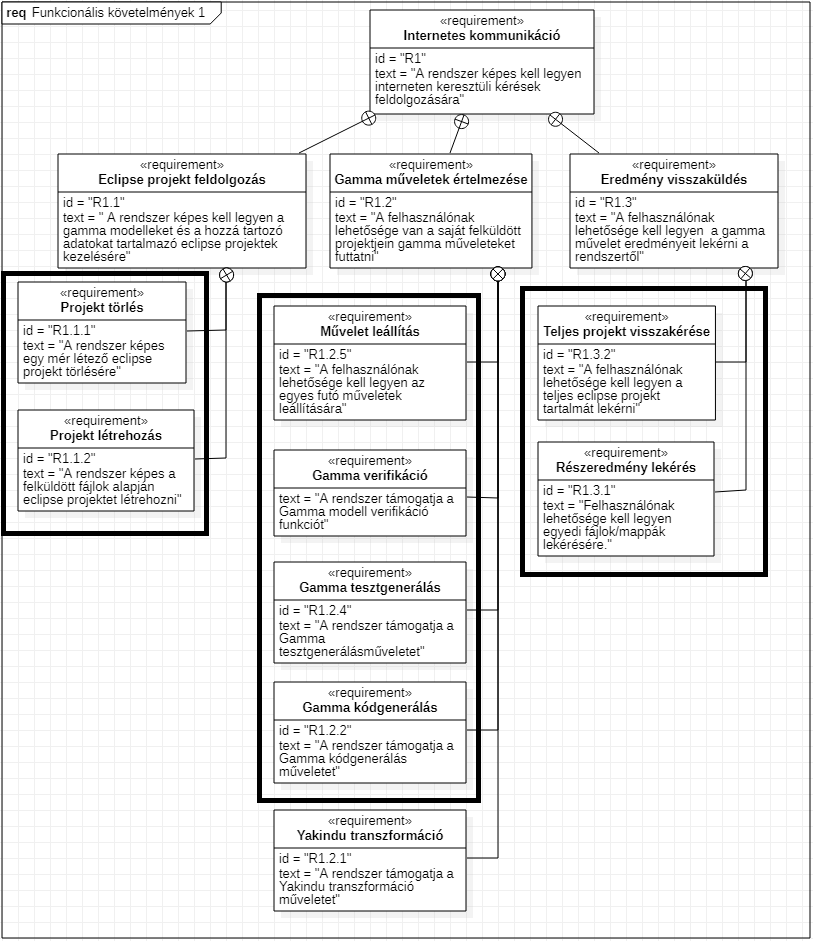
\includegraphics[width=\textwidth, keepaspectratio]{figures/requierments_placeholder_done.PNG}
	\caption{Teljesült funkcionális követelmények 1}
	\label{fig:requierments_placeholder_done}
\end{figure}
\begin{figure}[t]
	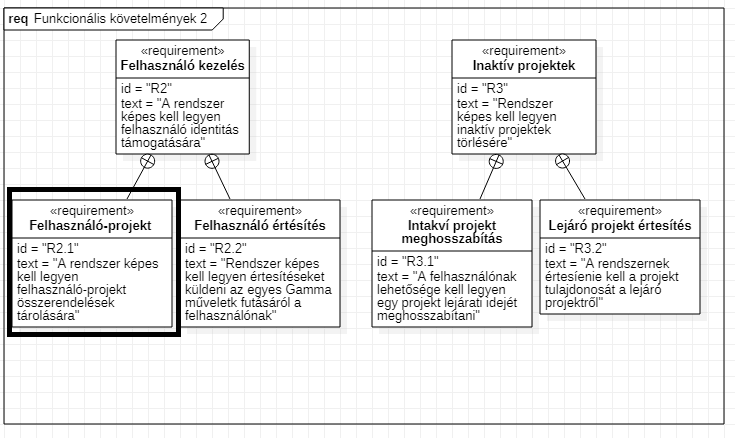
\includegraphics[width=\textwidth, keepaspectratio]{figures/requierments_2_done.PNG}
	\caption{Teljesült funkcionális követelmények 2}
	\label{fig:requierments_2_done}
\end{figure}



% List of Figures, Tables
%~~~~~~~~~~~~~~~~~~~~~~~~~~~~~~~~~~~~~~~~~~~~~~~~~~~~~~~~~~~~~~~~~~~~~~~~~~~~~~~~~~~~~~
%\listoffigures\addcontentsline{toc}{chapter}{\listfigurename}
%\listoftables\addcontentsline{toc}{chapter}{\listtablename}


% Bibliography
%~~~~~~~~~~~~~~~~~~~~~~~~~~~~~~~~~~~~~~~~~~~~~~~~~~~~~~~~~~~~~~~~~~~~~~~~~~~~~~~~~~~~~~
\addcontentsline{toc}{chapter}{\bibname}
\bibliography{bib/mybib}


% Appendix
%~~~~~~~~~~~~~~~~~~~~~~~~~~~~~~~~~~~~~~~~~~~~~~~~~~~~~~~~~~~~~~~~~~~~~~~~~~~~~~~~~~~~~~

%\label{page:last}
\end{document}
